% GENERATED from paper/preprint.md by paper/tools/build_paper.py. DO NOT EDIT THE GENERATED TEX.
% Manuscript SHA256: 124addcae95cdb86d41f6e52f21e0ea62a6a35929b5696d55c1551adb580cf8b
% Options for packages loaded elsewhere
\PassOptionsToPackage{unicode}{hyperref}
\PassOptionsToPackage{hyphens}{url}
\documentclass{article}
\usepackage[preprint]{neurips_2026}
\usepackage[utf8]{inputenc}
\usepackage[T1]{fontenc}
\usepackage{xcolor}
\usepackage{amsmath,amssymb}
\usepackage{longtable,booktabs,array}
\usepackage{calc} % for calculating minipage widths
% Correct order of tables after \paragraph or \subparagraph
\usepackage{etoolbox}
\makeatletter
\patchcmd\longtable{\par}{\if@noskipsec\mbox{}\fi\par}{}{}
\makeatother
% Allow footnotes in longtable head/foot
\IfFileExists{footnotehyper.sty}{\usepackage{footnotehyper}}{\usepackage{footnote}}
\makesavenoteenv{longtable}
\usepackage{graphicx}
\makeatletter
\newsavebox\pandoc@box
\newcommand*\pandocbounded[1]{% scales image to fit in text height/width
  \sbox\pandoc@box{#1}%
  \Gscale@div\@tempa{\textheight}{\dimexpr\ht\pandoc@box+\dp\pandoc@box\relax}%
  \Gscale@div\@tempb{\linewidth}{\wd\pandoc@box}%
  \ifdim\@tempb\p@<\@tempa\p@\let\@tempa\@tempb\fi% select the smaller of both
  \ifdim\@tempa\p@<\p@\scalebox{\@tempa}{\usebox\pandoc@box}%
  \else\usebox{\pandoc@box}%
  \fi%
}
% Set default figure placement to htbp
\def\fps@figure{htbp}
\makeatother
\setlength{\emergencystretch}{3em} % prevent overfull lines
\providecommand{\tightlist}{%
  \setlength{\itemsep}{0pt}\setlength{\parskip}{0pt}}
\usepackage{bookmark}
\IfFileExists{xurl.sty}{\usepackage{xurl}}{} % add URL line breaks if available
\urlstyle{same}
\hypersetup{
  pdftitle={ArdEVO: Toward Task-General Intelligence with Persistent, Compounding Neuroevolution},
  hidelinks,
  pdfcreator={LaTeX via pandoc}}
\setcounter{secnumdepth}{-\maxdimen}

\title{ArdEVO: Toward Task-General Intelligence with Persistent, Compounding Neuroevolution}
\author{%
  John Gardner \\
  Ardea AI \\
  \texttt{john@ardea.io}
}
\date{}

\begin{document}
\maketitle
\begin{abstract}
Intelligence appears in many forms and substrates, making a complete hand specification of its mechanisms implausible. We investigate a narrower first-principles hypothesis: a task-general learning system should evolve reusable neural structure, preserve verified discoveries, and become cheaper to search as those discoveries compound. ArdEVO is a persistent neuroevolution system built around this hypothesis. Its orchestrator searches a typed library, refines known solutions, routes among frozen experts, evolves network topology, composes prior modules, and recursively decomposes tasks. Gradient descent trains weights inside each structural candidate; evolution controls topology. Verified networks return to a quality-diversity library, while below-threshold champions remain stepping stones.\\
We evaluate ArdEVO on Icarus, an 18-rung curriculum spanning Boolean functions, control traces, images, scientific modalities, abstract reasoning, and ARC-AGI under one differentiable support/query contract. A historical 400-task lower-ladder run demonstrates compounding: 234 encounters resolved from memory, and retained solutions formed five composition levels. A broader pre-change run completed 180 tasks but exposed substantial support-to-query gaps. A post-change cold canary then completed one task per rung in 6,925.5 task-seconds. It recorded held-out accuracy for 16 of 18 tasks, with mean 0.6626 versus mean support accuracy 0.8312, and grew a 23-entry, six-level library. Routed handoff and recursive recovery executed on wide tasks, but image and ARC results generalized poorly. ARC is cell-level accuracy, not an exact-grid solve.\\
These results support the viability of one persistent evolutionary loop across heterogeneous modalities. They do not establish task-general intelligence, baseline superiority, reliable upper-rung generalization, recursive self-improvement, or consciousness.
\end{abstract}

\section{1 Why Evolve Intelligence?}\label{1-why-evolve-intelligence}

The full spectrum of intelligence is too broad, internally varied, and substrate-dependent to expect a human designer to specify every useful mechanism directly. Human cognition is itself not a single smooth capability, and biological systems exhibit forms of sensing, control, memory, and collective behavior that do not map cleanly onto a human checklist. Systems assembled from manually selected mechanisms can be powerful, but their competence tends to follow the boundaries of the structures and objectives their designers anticipated. This motivates a different question: can a search process discover, retain, and recombine its own computational structure across tasks?

Evolution is an existence proof for accumulating functional structure without a complete top-down design. It operates through variation, selection, inheritance, and repeated reuse of prior structure. Neuroevolution translates part of that process into neural computation (Stanley and Miikkulainen, 2002; Stanley et al., 2019). The central hypothesis of ArdEVO is not that biological evolution should be copied literally. It is that three of its properties are useful engineering commitments:

\begin{enumerate}
\def\labelenumi{\arabic{enumi}.}
\tightlist
\item
  the representation must be able to grow rather than select only from a fixed catalog;
\item
  discoveries must persist beyond the task and run that produced them; and
\item
  later search must be able to reuse, alter, compose, or retire those discoveries.
\end{enumerate}

The long-term aim is a system that is not taught a fixed vocabulary of words, sounds, or visual objects, but can discover structures through which it learns to read, hear, and see. The present system does not reach that aim. It consumes supervised, differentiable tasks with human-provided input and output fields. What it tests is a prerequisite: whether one evolutionary process can operate across heterogeneous task shapes while preserving useful structure and exposing its own failures.

This framing differs from optimizing one model for one benchmark. ArdEVO treats the persistent library, rather than a final champion, as the durable product. A solution can be used as a frozen expert, embedded as a macro, placed inside a larger composition, or selected as a warm seed. Familiar work should become cheap; unfamiliar work should alter the future search distribution. We call this \textbf{compounding}. In the current paper, that term has a deliberately narrow meaning: retained artifacts reduce later search cost or provide structure that later search actually uses. It does not mean that the software rewrites itself, invents its own objectives, or improves without an external task stream.

The paper makes three contributions. First, it presents a complete persistent neuroevolution loop that combines structural evolution, gradient-trained weights, routed reuse, hierarchical composition, recursive decomposition, quality-diversity admission, and lifecycle decay under one task-independent interface. Second, it separates search-time support fitting from held-out query reporting and separates measured behavior from post-run engineering changes. Third, it reports evidence from several development eras, culminating in a July 15 canary that exercised the current cross-modal path while revealing that reusable support-fitting structure still does not yield reliable upper-rung generalization.

\section{2 Related Work}\label{2-related-work}

\subsection{2.1 Growing neural structure}\label{21-growing-neural-structure}

NEAT established a practical recipe for growing topology from minimal networks, protecting new structure through speciation, and aligning crossover with historical markings (Stanley and Miikkulainen, 2002). ArdEVO retains that lineage but assigns weights to a gradient inner loop, writes trained weights back into genomes, and makes a cross-task library the unit of inheritance. This division is Lamarckian in the engineering sense (Whitley et al., 1994): evolution proposes structure, learning evaluates and fills it, and the trained result can survive. The interaction is important because insufficient inner-loop training can cause evolution to discard a structurally promising candidate before its value becomes visible, an instance of the coupling studied by Hinton and Nowlan (1987).

Neural architecture search usually searches a predefined operation space using evolution, reinforcement learning, parameter sharing, or differentiable relaxation (Real et al., 2017, 2019; Liu et al., 2019; Elsken et al., 2019). ArdEVO instead asks whether reusable operations can themselves emerge from a growing graph library. It therefore avoids seeding convolution, attention, or recurrent-cell templates. This is not a claim of prior-free learning: the graph language, mutations, loss contract, curriculum, and resource budgets are all human choices. It is a narrower constraint against task-specific architectural primitives.

Indirect encodings provide a route to repeated structure. CPPNs and HyperNEAT generate large patterns from compact genomes (Stanley, 2007; Stanley et al., 2009), while Weight Agnostic Neural Networks evaluate how much function topology carries under shared weights (Gaier and Ha, 2019). ArdEVO uses direct graph growth in its main path, supports a generative initializer, and records shared-weight robustness as a diagnostic. Its composition strategy is related to CoDeepNEAT\textquotesingle s blueprint/module distinction (Miikkulainen et al., 2017), but its modules are executable, typed, previously trained networks rather than layer specifications.

\subsection{2.2 Stepping stones and reusable libraries}\label{22-stepping-stones-and-reusable-libraries}

Novelty search and quality-diversity methods preserve alternatives that objective-only search would discard (Lehman and Stanley, 2011; Mouret and Clune, 2015; Pugh et al., 2016). Go-Explore makes the related strategy of returning to a retained stepping stone before exploring again explicit (Ecoffet et al., 2021). ArdEVO applies these ideas at two timescales. Within evolution, novelty and wiring cost can participate in multi-objective selection. Across tasks, verified entries occupy behavioral niches, while executable below-threshold champions can seed later attempts.

Program-synthesis systems such as DreamCoder and Stitch build reusable libraries by compressing prior solutions (Ellis et al., 2021; Bowers et al., 2023). Voyager similarly uses a persistent skill library as an anti-forgetting mechanism in an embodied setting (Wang et al., 2023). ArdEVO shares the compounding objective but stores trained neural graphs and compositions rather than symbolic programs or generated code. Its library is both memory and a changing search substrate.

This places the work near open-ended and AI-generating-algorithm research (Clune, 2019; Stanley et al., 2017; Wang et al., 2019, 2020). The current system is not open-ended in the strong sense. Tasks, metrics, and budgets are externally supplied, and every durable artifact must pass a fixed verifier. The relevance is architectural: inheritance, stepping stones, and an expanding vocabulary are mechanisms by which a bounded system could later support a less bounded one.

\subsection{2.3 Routing, modularity, and continual learning}\label{23-routing-modularity-and-continual-learning}

Mixture-of-experts systems learn gates over specialist networks (Jacobs et al., 1991; Shazeer et al., 2017). Modular meta-learning, neural module networks, and soft layer ordering likewise search over reusable computation (Andreas et al., 2016; Alet et al., 2018; Meyerson and Miikkulainen, 2018). ArdEVO\textquotesingle s router differs in two ways. Experts are immutable entries accumulated by evolution, and a router score is diagnostic until its behavior is distilled into an executable composition that passes ordinary verification. This prevents a transient adapter from being counted as reusable knowledge.

Continual-learning systems protect weights, expand architectures, or maintain module pools to limit catastrophic forgetting (McCloskey and Cohen, 1989; Rusu et al., 2016; Veniat et al., 2021; Mendez and Eaton, 2021). ArdEVO accepts structural growth as the cost of avoiding destructive interference. Entries are immutable; replacement creates a new entry; references keep dependencies alive; and inactive routes and unreferenced entries can decay and retire. This moves forgetting from uncontrolled parameter drift to an explicit, inspectable lifecycle policy.

\section{3 Problem Setting and Honest Evaluation}\label{3-problem-setting-and-honest-evaluation}

\subsection{3.1 One contract across heterogeneous tasks}\label{31-one-contract-across-heterogeneous-tasks}

Icarus is an 18-rung curriculum expressed through one typed task contract. A field carries a tensor and descriptors for semantic axes, value type, class count, value range, and padding mask. A task contains support examples for search and a query split for held-out reporting. Descriptor-driven loss dispatch selects cross-entropy, binary cross-entropy, or mean squared error without inspecting the task\textquotesingle s name. Structural library signatures derive from field descriptors and widths rather than benchmark identity.

The rungs move from XOR and parity through two-spirals, control traces, MNIST and CIFAR, nine NAS-Bench-360 modalities, RAVEN/PGM-style reasoning, and ARC-AGI (Tu et al., 2022; Barrett et al., 2018; Chollet, 2019). Their flattened widths range from two inputs and one output to millions of inputs and hundreds of thousands of outputs. This diversity stresses more than predictive accuracy. It stresses initialization cost, adapter size, temporal execution, structured placement, routing, and whether one orchestration loop can remain valid as shapes change. The complete rung table appears in the technical supplement.

The ladder is a curriculum, not a proof of generality. It is ordered by intended difficulty, and its task distribution is designed by humans. A run over all rungs demonstrates interface and mechanism coverage only. Comparative capability requires matched baselines and repeated seeds.

\subsection{3.2 Support is for search; query is for evidence}\label{32-support-is-for-search-query-is-for-evidence}

Evolution, routing, composition, and admission use support data. The selected executable artifact receives a held-out query evaluation. \textbf{Held-out query accuracy is the primary reported metric.} Support accuracy is shown separately because it measures what search fit, not what generalized. A high support score can therefore produce an accepted runtime outcome while its query score remains poor. We report that discrepancy rather than retroactively redefining the outcome.

Metric availability is literal. A valid accuracy of zero is reported as \texttt{0.0000}. \texttt{N/A} means that no defensible measurement exists. In the July 15 canary, Psicov and PGM reached their deadlines before an executable parent could be evaluated, so neither support nor query accuracy is imputed. Aggregates exclude unavailable values and retain valid zeroes.

Structured tasks require additional caution. The July 15 ARC row records ordinary encoded support and held-out accuracy, but the archived task row contains no exact-grid, predicted-shape, coverage, or baseline fields. The support path also fell back to literal support accuracy. We therefore describe its 1.0 support and 0.20 query values as cell/sample-level evidence only. They do not constitute an ARC task-exact solve. The same rule applies to the July 12 ARC results, whose mean held-out cell accuracy was 0.5128 and whose best value was 0.84375.

\subsection{3.3 Evidence is tied to code era}\label{33-evidence-is-tied-to-code-era}

ArdEVO changed substantially between the archived campaigns. We use the artifacts as historical evidence, not as if all runs measured the current implementation.

\begin{longtable}[]{@{}
  >{\raggedright\arraybackslash}p{(\linewidth - 4\tabcolsep) * \real{0.3333}}
  >{\raggedright\arraybackslash}p{(\linewidth - 4\tabcolsep) * \real{0.3333}}
  >{\raggedright\arraybackslash}p{(\linewidth - 4\tabcolsep) * \real{0.3333}}@{}}
\toprule\noalign{}
\begin{minipage}[b]{\linewidth}\raggedright
Evidence era
\end{minipage} & \begin{minipage}[b]{\linewidth}\raggedright
Scope
\end{minipage} & \begin{minipage}[b]{\linewidth}\raggedright
What it can support
\end{minipage} \\
\midrule\noalign{}
\endhead
\bottomrule\noalign{}
\endlastfoot
July 5-6 lower-ladder studies & repeated tasks on rungs 1-6; dedicated two-spirals diagnostics & compounding behavior, marginal cost, and a representation/training case study under historical configurations \\
July 12 preflight & ten tasks on every rung, 180 total & broader pre-change performance and failure characterization \\
July 15 canary & one task on every rung, cold library, current method & functionality of the post-change path and one observational scorecard \\
\end{longtable}

The July 15 run is not a treatment arm for July 12. It uses a different task sample, task count, codebase, budgets, and library trajectory. Differences between their metrics cannot be assigned to any particular engineering change. Every result in this paper is one seed on one curriculum. The executable Git revision was not pinned contemporaneously in either canary, although configuration and artifacts were frozen.

\section{4 The Current ArdEVO Method}\label{4-the-current-ardevo-method}

\subsection{4.1 The persistent solve loop}\label{41-the-persistent-solve-loop}

Figure 1 summarizes the current task lifecycle. Given a task, the orchestrator first checks structurally compatible library entries. A verified hit can be returned immediately or given a bounded refinement budget. On a miss, the system escalates through routed reuse, a motif-derived grammar, direct topology evolution, and evolution over compositions. If the parent remains unsolved, decomposition creates smaller typed subtasks, solves them recursively, and then retries the parent with the new components available. A verified winner is offered to the library; an executable champion below the acceptance threshold can be retained as a stepping stone.

\pandocbounded{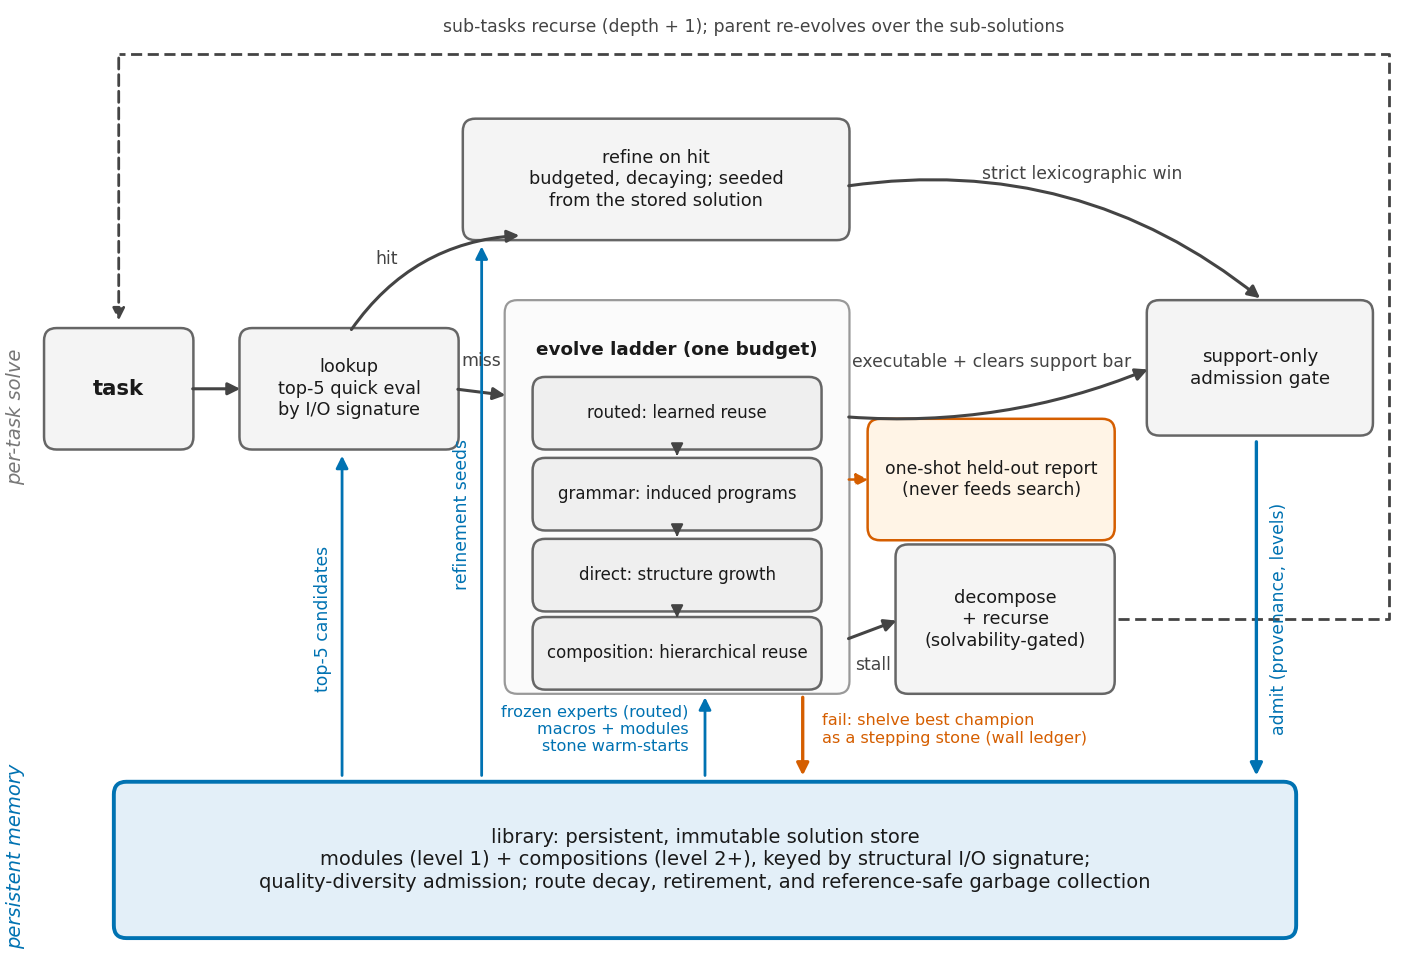
\includegraphics[keepaspectratio]{../../figures/fig1_ladder.png}}

\emph{Figure 1: The ArdEVO task loop. Search begins from persistent memory, escalates through reuse and structural search, may recurse over typed subtasks, and returns verified artifacts to a lifecycle-managed library. Held-out query evaluation occurs only after search selects an executable artifact.}

This is an orchestration policy, not a cascade of benchmark-specific solvers. Strategies share a task descriptor and a cumulative budget. Unused generations carry forward. Deadlines are checked at durable seams, and each strategy records its own timing, resource estimate, and failure stage. A graceful Escape request follows the same finalization path as normal completion, producing the rolling checkpoint and final reports rather than treating the run as a crash.

\subsection{4.2 Evolving structure and training weights}\label{42-evolving-structure-and-training-weights}

Direct search begins with a minimal, sparse, factored, or generatively initialized graph. Mutations add and remove nodes and connections, alter activations and aggregation, introduce recurrence or refinement depth, and reference frozen library modules. Speciation protects structural innovations; crossover uses historical identity; multi-objective selection can combine support accuracy, behavioral novelty, and connection cost. Gradient descent trains candidate weights, and Lamarckian writeback returns trained values to the genome.

The split is deliberate. Pure weight mutation was ineffective even on low rungs in early experiments, while gradient training provides a common optimizer across field types. Evolution is reserved for discrete structure and search strategy. Shared-weight samples measure whether a topology carries useful function independently of its fitted weights, but are a diagnostic and quality signal rather than a substitute for held-out evaluation.

Composition evolution searches graphs whose vertices can be prior modules. Fixed port maps join mismatched interfaces with compact axis- and shape-derived index runs. Four generic maps are available: output slices, input subsets, time windows, and spatial patches. Execution gathers selected values and scatters them into the target placement. These maps remain fixed through serialization, mutation, crossover, writeback, nested composition, and resource estimation. This replaced dense, mostly zero glue that made wide decomposition both expensive and role-limited.

\subsection{4.3 Routing and executable handoff}\label{43-routing-and-executable-handoff}

The routed strategy learns sparse top-k paths over the complete set of library vertices. Experts remain frozen; small gate embeddings remain resident; wide input adapters, output heads, and selected expert state load on demand. Router format v2 shards those components so state scales with active use rather than requiring every wide tensor to remain resident.

A router score alone is never an admission. The selected pathway must distill into an executable composition. If distillation falls below the acceptance threshold but still produces a valid artifact, that artifact is deduplicated and handed to ordinary composition as a warm seed. The strategy ledger records router score, distilled score, their gap, handoff count, and any recovery score. Metric-only router results remain diagnostics. This distinction matters in the canary: routed paths often identified useful experts, while parent execution still required composition or decomposition to recover.

\subsection{4.4 Persistent memory, identity, and decay}\label{44-persistent-memory-identity-and-decay}

Library entries are immutable modules or compositions. They are indexed by structural signatures and behavior niches, and may refer to older entries as dependencies. Two identities serve different purposes. Content identity prevents duplicate serialized artifacts; topology identity ignores fitted parameter values and prevents exact structural proposals from consuming repeated evaluation budget. The topology tabu is scoped to the relevant search context so that a known structure can still be retrained when the intended experiment requires it.

Usage is not permanent entitlement. Router edges decay when they stop carrying traffic. Vertices whose routes disappear become inactive; inactive, unreferenced library entries can then retire after their configured grace period. Garbage collection removes only artifacts that are both retired and unreachable. The full overmind render preserves historical cards, while the pruned render packs current entries into the same eight-column grid for direct comparison. This two-stage policy makes removal algorithmic and auditable rather than allowing the library to grow without pressure.

\subsection{4.5 Reporting and provenance}\label{45-reporting-and-provenance}

The runtime display reports conceptual stage transitions and always closes each task with support and held-out query status. Machine-readable attempts retain the detailed metrics without flooding the terminal. Every durable summary update atomically refreshes a schema-versioned JSON report, a Markdown report, and a per-rung CSV. Missing and zero metrics remain distinct.

Runs snapshot the source and effective configurations with hashes. External archives use content-addressed manifests so unchanged run, library, and router objects are uploaded once; restore verifies hashes before atomic installation. The technical report records resource accounting, historical incidents, and artifact provenance in detail.

\section{5 Evidence Eras and Experimental Protocol}\label{5-evidence-eras-and-experimental-protocol}

All reported campaigns used seed 0 on one Apple M4 Max with 128 GB unified memory and CPU-resident search. The total recorded task wall clock across the cited campaigns is approximately 21.9 hours. This is an accounting total, not a hardware-normalized compute comparison.

The historical lower-ladder run began from an empty library and interleaved 400 task encounters over rungs 1-6. Its configuration predates the current full-method profile, but it remains the clearest repeated-task test of compounding because each solved family appears many times. The two-spirals studies used repeated assaults and controlled configuration flips to diagnose why retained structure did not cross the acceptance threshold.

The July 12 preflight scheduled ten tasks from each of the 18 rungs. It completed all 180 tasks in 49,311.5 seconds and 3,987 generations. Outcomes were 74 evolved, 64 failed, 36 library hits, 4 refinements, and 2 decompositions. Held-out metrics were recorded for 137 tasks. The run created 84 entries and retained 69 after garbage collection. It predates compact port maps, executable routed handoff, router v2 sharding, lifecycle decay, topology tabu, and the current reporting semantics. We use it to characterize scale and generalization gaps, not to validate those later changes.

The July 15 canary used the current canary profile, a cold library, and one task per rung. It was intended to exercise the deepest available path on each modality while bounding total runtime. It completed 18 of 18 tasks, ran 720 generations, and recorded 6,925.5 task-seconds. The one-task sample makes per-rung results illustrative rather than estimates of rung-level performance.

In all result tables, runtime outcome labels describe what the orchestrator did under its support-side rules. They are not substitutes for query success. For example, a task may be recorded as \texttt{evolved} because an executable support-side champion was admitted while its held-out accuracy is low. We therefore lead with query results and report mechanisms separately.

\section{6 Measured Results}\label{6-measured-results}

\subsection{6.1 Repeated tasks compound on the lower ladder}\label{61-repeated-tasks-compound-on-the-lower-ladder}

The historical cold 400-task run attempted every scheduled task, consumed 15,590 generations and 10,198 task-seconds, and ended with 49 entries before garbage collection and 35 after. Rungs 1, 2, 4, and 5 solved 266 of 267 encounters under that run\textquotesingle s historical acceptance semantics. Rungs 3 and 6 remained unsolved at best metrics 0.901 and 0.900 against a 0.95 threshold.

The relevant result is the change in marginal work. Of 400 encounters, 217 were direct library hits and 17 were hits that strictly improved under bounded refinement. Only 32 encounters required a fresh evolutionary solve. Forty-six refinement attempts yielded 17 improvements; 188 later refinement opportunities were skipped by the decayed cooldown. The final retained graph contained live entries through level 5, showing that compositions of compositions arose without a prescribed depth schedule. Every later two-spirals or MNIST-family assault warm-started from a retained stepping stone.

\pandocbounded{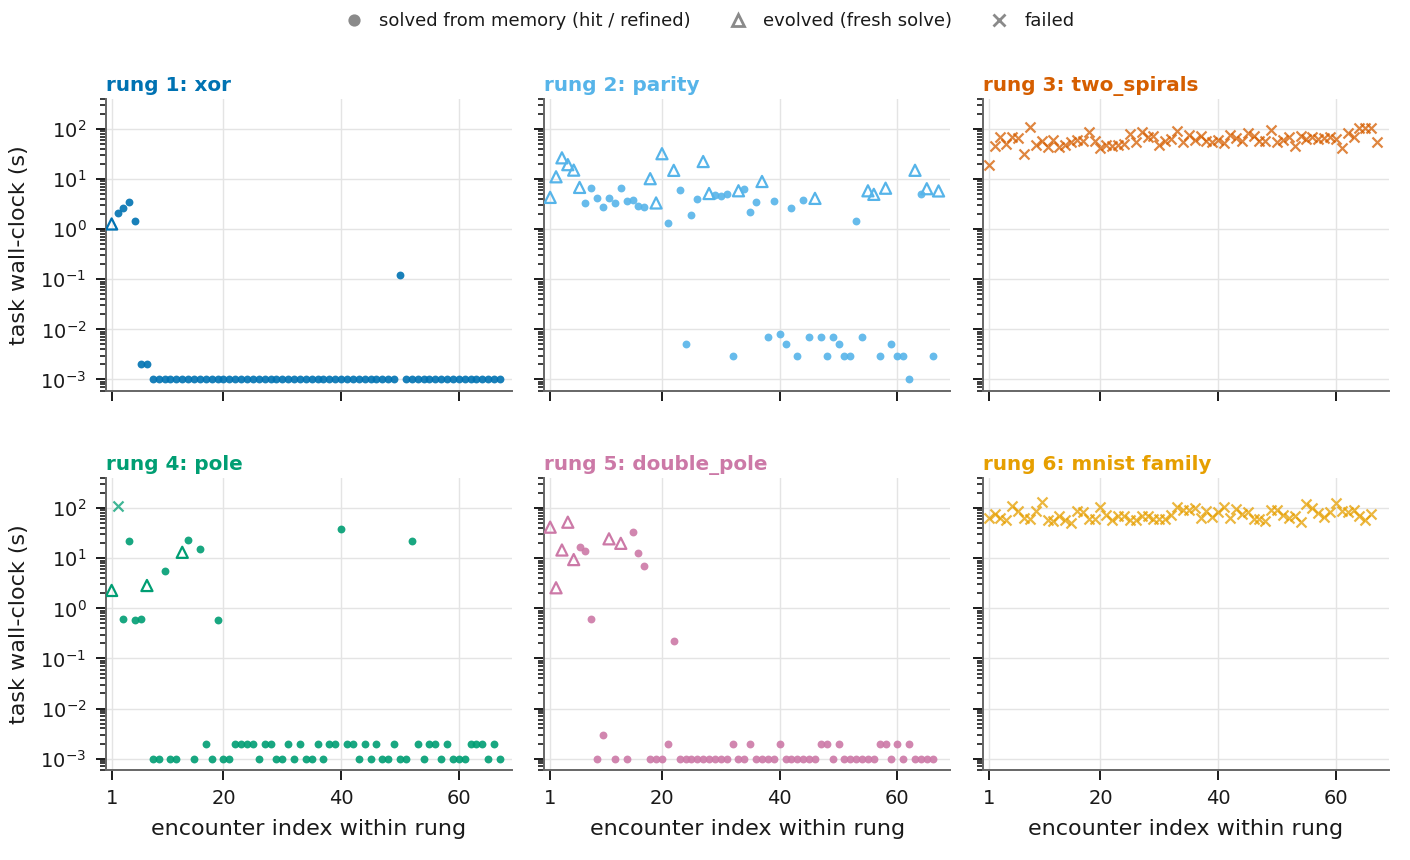
\includegraphics[keepaspectratio]{../../figures/fig2_cost.png}}

\emph{Figure 2: Historical marginal task cost in the cold 400-task run. Filled points are encounters resolved from memory, open triangles are fresh solves, and crosses are failures. Repeated solved families fall from evolutionary search to millisecond or bounded-refinement retrieval; unsolved families continue to pay search cost.}

This is evidence that persistent memory can reduce repeated-task cost. It is not yet a clean causal estimate of the entire library mechanism because the run has one seed and no matched fresh-per-task control. Those controls remain part of the planned campaign.

\subsection{6.2 The broad pre-change run exposed generalization gaps}\label{62-the-broad-pre-change-run-exposed-generalization-gaps}

The July 12 preflight demonstrated that one historical loop could execute all 18 rungs, but support fitting frequently failed to transfer. ARC support averaged 0.9994 while held-out cell accuracy averaged 0.5128. PGM support averaged 1.0 while query averaged 0.1077. Image rungs also showed large gaps. The run\textquotesingle s 48 deadline events concentrated in upper rungs, and its router state grew to 5.3 GiB. These observations motivated compact parent wiring, explicit routed handoff, sharded router storage, and more literal reporting.

The scientific conclusion is negative but useful: a reusable support-fitting system did not thereby acquire reliable upper-rung generalization. The run also provides no matched baseline, exact-grid ARC metric, or pinned executable revision. Its full 18-row table and postmortem appear in the technical supplement.

\subsection{6.3 The current-method canary exercised the current path}\label{63-the-current-method-canary-exercised-the-current-path}

The July 15 run recorded held-out accuracy for 16 of 18 root tasks. Across those 16, mean query accuracy was 0.6626. Mean support accuracy across available root measurements was 0.8312, and the mean paired support-minus-query gap was 0.1686. A zero-valued spherical query is included; Psicov and PGM are unavailable rather than treated as zero. Runtime outcomes were 9 evolved, 2 decomposed, and 7 failed.

\pandocbounded{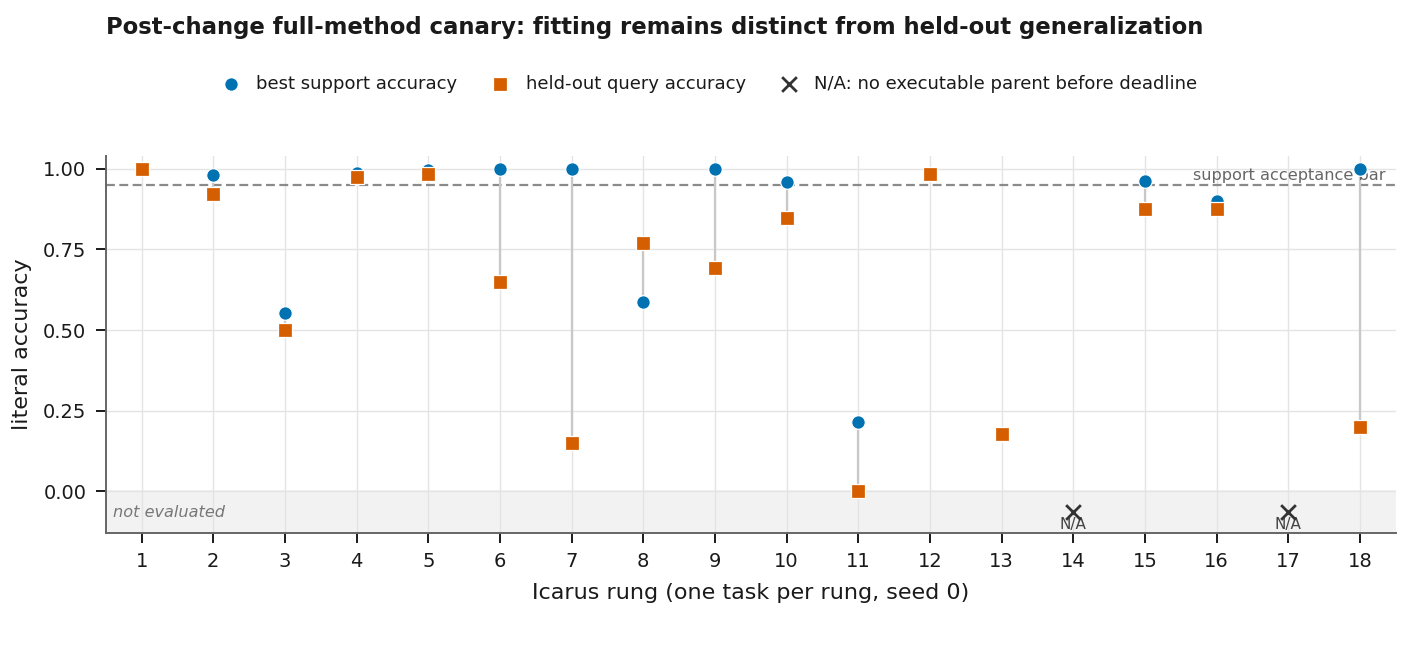
\includegraphics[keepaspectratio]{../../figures/fig7_canary.png}}

\emph{Figure 3: July 15 support and held-out query accuracy by rung. A zero query score is plotted as a valid measurement. Psicov and PGM are marked unavailable because their deadlines arrived before executable parent evaluation. Values are one task per rung, not rung-level estimates.}

The lower and control rungs generalized strongly in this sample: XOR reached 1.0 query accuracy; parity 0.9231; pole 0.9750; and double-pole 0.9833. Cosmic was the strongest wide structured example, with 0.9848 support and 0.9837 query accuracy after decomposition. FSD50K recorded 0.9615 support and 0.8742 query, and DeepSEA 0.8998 and 0.8761.

The gaps remain the dominant result. MNIST recorded 1.0 support and 0.65 query. CIFAR recorded 1.0 and 0.15. Satellite recorded 1.0 and 0.6923. The ARC task recorded 1.0 support and 0.20 held-out cell/sample accuracy. No exact-grid, shape, coverage, or baseline measurement was present, so this is not an ARC solve. Two-spirals remained near chance at 0.5515 support and 0.50 query. Spherical\textquotesingle s valid query value was 0.0. Psicov and PGM produced neither support nor query measurements before their deadlines.

The cold library grew from 0 to 23 entries: 7 modules and 16 compositions, with one level-6 entry. No entry was retired or collected. The run recorded no root refinement outcome and no root library-hit outcome, as expected from one cold encounter per rung, so those current mechanisms were not evaluated by this canary.

\subsection{6.4 What the mechanism traces show}\label{64-what-the-mechanism-traces-show}

Routed-to-composition handoff occurred five times at root level; two roots, Cosmic and ARC, later recorded recovery results. Including recursive subtasks, the run recorded nine handoffs and five recoveries. Cosmic and ARC ended as decomposition outcomes, demonstrating that compact selection/placement, recursion, routed diagnostics, and executable parent recovery can coexist on very wide structures. This is mechanism execution evidence, not evidence that routing caused their query scores.

Five root tasks hit a deadline marker. Deadline enforcement is cooperative at generation and strategy seams, so an expensive unit can overshoot its nominal boundary before control returns. Psicov and PGM ended with \path{time_limit_before_evaluation}, which is why their metrics are unavailable. Three route edges expired during the run, exercising edge decay, but no router vertex or library entry reached retirement. Router v2 persisted a small core plus shards, demonstrating the storage layout; eager-versus-sharded parity is established by tests rather than by this scorecard.

\section{7 Observed, Tested, and Pending Mechanisms}\label{7-observed-tested-and-pending-mechanisms}

The distinction between an implemented mechanism and an empirically supported mechanism is essential in a rapidly changing research system.

\begin{longtable}[]{@{}
  >{\raggedright\arraybackslash}p{(\linewidth - 2\tabcolsep) * \real{0.5000}}
  >{\raggedright\arraybackslash}p{(\linewidth - 2\tabcolsep) * \real{0.5000}}@{}}
\toprule\noalign{}
\begin{minipage}[b]{\linewidth}\raggedright
Mechanism
\end{minipage} & \begin{minipage}[b]{\linewidth}\raggedright
Current evidence status
\end{minipage} \\
\midrule\noalign{}
\endhead
\bottomrule\noalign{}
\endlastfoot
Persistent lookup and refinement & Observed repeatedly in the historical lower-ladder run; not exercised at root level by the cold July 15 one-task schedule \\
Hierarchical compositions & Observed through level 5 historically and level 6 in July 15 \\
Compact port maps and recursive placement & Executed in July 15 decomposition paths; exact gather/scatter behavior is regression-tested \\
Routed executable handoff & Observed in July 15 traces, including recoveries; causal performance benefit unmeasured \\
Router v2 sharding & Persisted in July 15; numerical parity and v1 migration are regression-tested \\
Route and library decay & Three route edges expired; vertex retirement, entry retirement, and GC were not exercised in July 15 and remain test-backed \\
Topology tabu and duplicate suppression & Implemented and regression-tested; July 15 counters show no topology census, so no canary compute saving is claimed \\
Motif discovery & Raw historical census is descriptive; null-graph and counterfactual labels are implemented, but July 15 produced no discovery study \\
Content-addressed external archives & Deduplication, verified restore, and v1 compatibility are test-backed; not a predictive result \\
Graceful Escape shutdown and paired renders & Operational features covered by tests; the completed July 15 run did not need graceful shutdown \\
\end{longtable}

The current motif vocabulary deserves particular restraint. Frequent subgraphs are useful grammar candidates, but frequency alone is not architectural discovery. The discovery pipeline now compares candidates with 64 deterministic label/degree-preserving null graphs, independent lineage support, within-signature performance, robustness, and reuse. Candidates must be locked from support/library evidence before query results are read. A candidate is \texttt{observed} only with structural surprise and positive performance association, \texttt{functional} only after a frozen edge knockout exceeds matched controls, and \texttt{replicated} only after functional evidence appears in two independent lineage roots. No new cell, convolution, or architectural invention is claimed here.

The next evidentiary step is not another one-task canary. It is the pre-registered, multi-seed full-cluster and ablation campaign: matched full versus no-library, no-routing, no-decomposition, no-hierarchy, and no-refinement arms; fresh-per-task controls; and external MLP, NEAT, WANN-style, and random-structure baselines under comparable budgets. The repository contains the runners and configurations, but tooling is not a result.

\section{8 Discussion}\label{8-discussion}

\subsection{8.1 What the evidence supports}\label{81-what-the-evidence-supports}

The strongest claim is architectural. One persistent system executed a common task contract from XOR to ARC, grew a multi-level library, used prior entries as routed experts and composition components, recursively decomposed wide tasks, and preserved enough state to make later search structurally different from earlier search. On repeated lower-rung families, memory reduced marginal task cost by orders of magnitude. The July 15 canary shows that the current method still executes after substantial changes to parent wiring, routed handoff, persistence, and lifecycle management.

This matters because task-general search needs more than a learner that can be reset for each benchmark. It needs an inheritance mechanism. ArdEVO offers one concrete answer: immutable neural artifacts, typed interfaces, verified composition, and explicit decay. The library makes accumulated structure inspectable and prevents new training from silently overwriting old solutions.

\subsection{8.2 What the evidence does not support}\label{82-what-the-evidence-does-not-support}

Cross-modal execution is not cross-modal mastery. The image and ARC gaps show that high support accuracy can coexist with weak held-out behavior. Reusable structure has so far amplified fitting more reliably than generalization. The current system also depends on a human curriculum, supervised targets, descriptor-defined losses, and externally selected acceptance thresholds. It has not learned its own task distribution or evaluation criteria.

The no-task-specific-primitives constraint creates a real tradeoff. Supplying convolution or a Fourier basis would likely improve particular rungs, but would answer a different question. ArdEVO instead searches for reusable primitives through generic graph operations, geometry, composition, and selection pressure. That choice makes negative results central: if repeated structure remains expensive or candidate training is too short to reveal a good genotype, the system must expose the failure rather than hide it behind a hand-built module. The two-spirals case study in the supplement is one example.

\subsection{8.3 Recursive improvement, narrowly construed}\label{83-recursive-improvement-narrowly-construed}

Persistent evolution creates a natural route to cumulative improvement: discoveries change the components, warm starts, and search paths available to subsequent tasks. In that limited sense, the process is recursively productive. The current implementation is not recursive self-improvement in the stronger sense used for systems that modify their own code, objectives, training algorithm, evaluator, or task generator. It evolves neural artifacts inside a fixed program. Claims beyond that boundary require a different experiment and substantially stronger safety analysis.

\subsection{8.4 Long-horizon motivation: agency and consciousness}\label{84-long-horizon-motivation-agency-and-consciousness}

The broader research motivation is artificial agency capable of developing rich internal object representations and, eventually, properties associated with subjectivity or consciousness. Evolution is relevant because biological agency and experience arose through cumulative adaptation rather than direct mechanism-by-mechanism engineering. A system that can discover its own perceptual and cognitive primitives may therefore be a more plausible component of that long-range program than one whose entire ontology is specified in advance.

Nothing in the present experiments measures qualia, objectness, selfhood, sentience, or consciousness. Benchmark accuracy, persistent memory, autonomous topology growth, and even future recursive self-modification would not by themselves establish any of those properties. ArdEVO should be evaluated here as a bounded search and memory system. Consciousness is a motivating destination, not an empirical contribution of this paper, and complementary systems and operational measures would be required before the question becomes scientifically testable.

\section{9 Limitations}\label{9-limitations}

\textbf{Single seed and curriculum dependence.} All reported campaigns use seed 0. Repeated encounters within one run are not independent samples, and the ladder ordering influences what enters the library. Confidence intervals, curriculum randomization, and matched cold/warm controls are pending.

\textbf{No matched external baselines.} ArdEVO has not yet been compared under equal budgets with a fixed MLP, canonical NEAT, WANN-style search, or random topology search on this contract. The current evidence supports internal behavior claims, not superiority.

\textbf{Historical/current boundary.} July 12 predates many current mechanisms. July 15 uses one task per rung and cannot isolate which change affected any metric. Neither canary pins an executable Git revision. Configuration hashes and archived artifacts reduce but do not remove this reproducibility gap.

\textbf{Generalization and metric limits.} The mean July 15 support-query gap was 0.1686, with severe image and ARC failures. ARC is reported only at the encoded cell/sample level, not exact-grid. Psicov and PGM have no root metrics. Task-specific baselines and structured shape/coverage fields were not recorded contemporaneously.

\textbf{Mechanism coverage.} July 15 did not exercise root library hits, refinement, topology duplicate counters, vertex retirement, library retirement, garbage collection, or motif counterfactuals. Those features are supported by tests or historical runs, not by this canary.

\textbf{Resource and deadline semantics.} Very wide adapters and compositions remain expensive. Cooperative deadlines can overshoot inside a generation. Router sharding reduces residency but does not reduce the mathematical width of a selected adapter or head.

\textbf{Bounded objective.} The system learns supervised mappings under human-defined descriptors and losses. It does not choose its own goals, operate an open-ended environment, rewrite its implementation, or provide evidence about consciousness.

\section{10 Conclusion}\label{10-conclusion}

ArdEVO begins from a simple premise: if intelligence cannot be specified mechanism by mechanism, a useful research system should search for its own structure and preserve what it finds. The resulting architecture couples topology evolution with gradient-trained weights, places verified neural artifacts in persistent memory, composes and routes those artifacts across tasks, and retires them through explicit lifecycle rules.

The evidence is promising and incomplete. Repeated lower-rung tasks became dramatically cheaper after their first solution, and multi-level reuse emerged. A broad historical run exposed serious support-to-query gaps. The July 15 current-method canary completed every rung, exercised routed handoff and recursive parent recovery, and grew a six-level library, while again showing weak generalization on images and ARC. That combination is the honest result: the persistent evolutionary substrate works across modalities, but it has not yet turned accumulated structure into reliable task-general competence.

The path forward is empirical. Multi-seed ablations must isolate which memory and search mechanisms matter; external baselines must establish whether evolution earns its cost; exact structured metrics must replace proxies; and future systems must distinguish cumulative library search from genuine self-modification. ArdEVO provides a testable platform for those questions, not their final answer.

\begin{center}\rule{0.5\linewidth}{0.5pt}\end{center}

\section{Acknowledgments}\label{acknowledgments}

The Icarus dataset is generated and maintained separately at github.com/ArdeaAI/Icarus-Dataset. Portions of the engineering were carried out with AI pair-programming assistance; all design decisions, constraints, and evaluations are the author\textquotesingle s.

\begin{center}\rule{0.5\linewidth}{0.5pt}\end{center}

\section{Technical Supplement}\label{technical-supplement}

This supplement accompanies \textbf{ArdEVO: Toward Task-General Intelligence with Persistent, Compounding Neuroevolution}. It retains the extended task contract, method details, historical experiments, complete rung tables, engineering postmortems, and reproducibility notes that are intentionally compressed in the conference core. Claims inherit the evidence boundary stated in the core: historical runs describe the code that produced them, current mechanisms are not credited with retroactive effects, and regression-tested behavior is not presented as measured campaign performance.

\section{Appendix A: Icarus Task Contract}\label{appendix-a-icarus-task-contract}

\subsection{A.1 Fields, tasks, and encoders}\label{a1-fields-tasks-and-encoders}

A \textbf{Field} contains a tensor plus the descriptors required to interpret it: semantic \texttt{axes} drawn from EXAMPLE, CHANNEL, TIME, HEIGHT, WIDTH, DEPTH, and EXTRA; a value type drawn from BINARY, CATEGORICAL, MULTILABEL, CONTINUOUS, and ORDINAL; a class count where applicable; an optional continuous range; and an optional padding mask. A \textbf{Task} contains non-empty support and query lists of input/output field pairs. Authoritative native splits are preserved. Other tasks receive deterministic splits from a stable task-derived seed.

Loss dispatch uses the output descriptor rather than the benchmark name. Categorical and ordinal fields use cross-entropy, binary and multilabel fields use binary cross-entropy with logits, and continuous fields use mean squared error. Masks weight every path consistently. The Level0 encoder flattens fields to \texttt{{[}batch,\ width{]}}, normalizes continuous values, and clears padded positions. Temporal encoding reconstructs the TIME axis and is equivalent to Level0 when the time extent is one.

Library signatures derive from value type, semantic axes, and flattened width. They deliberately exclude the task name and rung. This permits structural compatibility across datasets while preventing benchmark labels from becoming lookup keys. It does not guarantee semantic transfer between same-shaped tasks; every candidate is re-evaluated on support before use.

\subsection{A.2 Complete rung inventory}\label{a2-complete-rung-inventory}

\begin{longtable}[]{@{}
  >{\raggedleft\arraybackslash}p{(\linewidth - 8\tabcolsep) * \real{0.2000}}
  >{\raggedright\arraybackslash}p{(\linewidth - 8\tabcolsep) * \real{0.2000}}
  >{\raggedleft\arraybackslash}p{(\linewidth - 8\tabcolsep) * \real{0.2000}}
  >{\raggedright\arraybackslash}p{(\linewidth - 8\tabcolsep) * \real{0.2000}}
  >{\raggedright\arraybackslash}p{(\linewidth - 8\tabcolsep) * \real{0.2000}}@{}}
\toprule\noalign{}
\begin{minipage}[b]{\linewidth}\raggedleft
Rung
\end{minipage} & \begin{minipage}[b]{\linewidth}\raggedright
Family
\end{minipage} & \begin{minipage}[b]{\linewidth}\raggedleft
Available tasks
\end{minipage} & \begin{minipage}[b]{\linewidth}\raggedright
Flattened input to output
\end{minipage} & \begin{minipage}[b]{\linewidth}\raggedright
Role in the ladder
\end{minipage} \\
\midrule\noalign{}
\endhead
\bottomrule\noalign{}
\endlastfoot
1 & XOR & 1 & BINARY 2 to BINARY 1 & smallest topology-growth test \\
2 & parity n4-n8 & 9 & BINARY up to 8 to BINARY 1 & discrete generalization \\
3 & two-spirals & 1 & CONTINUOUS 2 to CATEGORICAL 2 & nonlinear representation wall \\
4 & pole & 39 & CONTINUOUS 4 per step to 1 & temporal control traces \\
5 & double-pole & 39 & CONTINUOUS 6 per step to 2 & harder temporal traces \\
6 & MNIST / Fashion-MNIST & 1,200 & CONTINUOUS 784 to CATEGORICAL 10 & first image statistics \\
7 & CIFAR & 1,000 & CONTINUOUS 3,072 to CATEGORICAL 10 & wider image statistics \\
8 & ECG & 1,287 & CONTINUOUS 1,000 to CATEGORICAL 4 & NAS-Bench-360 temporal task \\
9 & Satellite & 15,625 & CONTINUOUS 46 to CATEGORICAL 24 & NAS-Bench-360 temporal task \\
10 & NinaPro & 62 & CONTINUOUS 832 to CATEGORICAL 18 & NAS-Bench-360 temporal task \\
11 & Spherical & 938 & CONTINUOUS 10,800 to CATEGORICAL 100 & wide spherical image task \\
12 & Cosmic & 512 & CONTINUOUS 65,536 to BINARY 65,536 & dense structured output \\
13 & Darcy Flow & 32 & CONTINUOUS 177,241 to CONTINUOUS 177,241 & dense field regression \\
14 & Psicov & 58 & CONTINUOUS 271k to at least 13.97M to CONTINUOUS 4.8k to at least 245k & variable, extremely wide structures \\
15 & FSD50K & 12,529 & CONTINUOUS 5,632 to MULTILABEL 200 & audio multilabel task \\
16 & DeepSEA & 3,489 & CONTINUOUS 4,000 to MULTILABEL 36 & temporal genomics task \\
17 & RAVEN / PGM & 23,294 & CONTINUOUS 409,600 to CATEGORICAL 8 & abstract relational reasoning \\
18 & ARC-AGI & 800 & CATEGORICAL 900 to CATEGORICAL 9,000 & structured program-induction target \\
\end{longtable}

Counts and widths were enumerated from the published dataset during the historical evidence freeze. The Psicov range is intentionally open-ended: the July 12 run observed a 13,966,425-input by 245,025-output task beyond the earlier probe range. Flattened widths describe the library-facing Level0 view; temporal substrates recover step structure where applicable.

The dataset is generated in a separate repository and published as \path{Ardea/Icarus-dataset}. ArdEVO vendors only the loader/encoder runtime. Rungs 4 and 5 originate from policy rollouts but are stored and evaluated as supervised traces. No interactive environment is present in the consumer. The rung scheduler is checkpointable and normally interleaves rungs so that library state changes between families.

\subsection{A.3 Structured outputs and metric availability}\label{a3-structured-outputs-and-metric-availability}

Variable-size structured targets require alignment between the support-derived head and query target. Generic tasks use a fixed-width masked representation. ARC support and query grids are placed in a two-dimensional canvas, and a separate support-fitted shape mechanism can report predicted dimensions and coverage when those fields are enabled. Unrepresented target cells count as incorrect.

Neither the July 12 nor July 15 ARC artifact contains a contemporaneous exact-grid result. The July 15 root row also lacks task-specific shape, coverage, and baseline fields. Its reported \texttt{support\_accuracy\ =\ 1.0} and \texttt{report\_metric\ =\ 0.20} are literal encoded-cell/sample accuracies. Any table or figure that calls this an ARC solve would be false. \texttt{N/A} has a similarly strict meaning: the evaluator had no executable root artifact from which to obtain the metric. It is never a rendered form of zero.

\section{Appendix B: Current Search and Memory System}\label{appendix-b-current-search-and-memory-system}

\subsection{B.1 Orchestration state machine}\label{b1-orchestration-state-machine}

The current root task sequence is:

\texttt{lookup\ -\textgreater{}\ optional\ refinement\ -\textgreater{}\ routed\ reuse\ -\textgreater{}\ grammar\ -\textgreater{}\ direct\ evolution\ -\textgreater{}\ composition\ evolution\ -\textgreater{}\ decomposition/retry\ -\textgreater{}\ admission\ or\ stepping\ stone}

Each stage consumes part of a cumulative generation and wall-time ledger. A strategy can return a verified accepted artifact, an executable below-threshold artifact, a diagnostic metric without an artifact, a resource decline, or a failure. Only executable artifacts may seed later structural stages or enter the library. A router score without successful distillation remains diagnostic.

Recursive tasks use the same state machine at a deeper depth. Decomposition is considered only when the remaining budget and operator-specific solvability checks justify it. A parent is not counted as solved merely because its subtasks solve. Newly admitted subtask artifacts expand the module pool, after which the parent must execute and verify.

Every attempt records outcome, strategy, generation count, support metric, held-out status at the root, stage timing, failure stage, candidate size, resource estimates, and strategy-specific metrics. Run summaries and checkpoints are replaced atomically at every durable boundary. A graceful Escape request is checked through the same cooperative seams and uses normal finalization; Ctrl-C remains a crash path.

\subsection{B.2 Graph genome and phenotype}\label{b2-graph-genome-and-phenotype}

The leaf representation extends a NEAT-lineage graph. Node genes carry activation and aggregation behavior, recurrent state where enabled, iterative refinement depth, and optional references to immutable library entries. Connection genes carry historical identity, endpoint identity, enablement, and trainable weight state. Innovation numbering aligns crossover and allows speciation distance to track structural change.

Mutations include adding and removing nodes or connections, changing activation and aggregation, toggling recurrence, changing refinement depth, geometric rewiring, and inserting library modules. Self-adaptive variants mutate and inherit their own operator rates. Initialization can be minimal, factored, sparse, or generated from a compact pattern-producing network. These are generic graph operations; none is a prebuilt convolution, attention block, or benchmark-specific cell.

The trainer owns weights. Candidate graphs are differentiated with respect to the support objective, and trained weights write back into the genome. Direct and composition populations can use different schedules and population execution paths while sharing the field-driven loss contract. Scheduled training, population batching, and device selection are configuration choices, not separate task solvers.

The evaluator reports trained support accuracy and loss, optional shared-weight samples, behavior descriptors, and structural size. Shared-weight robustness is inspired by weight-agnostic evaluation: every trainable weight receives the same scalar for each sample, and the best/mean response estimates how much function is expressed by topology alone. It is useful for diagnostics and archive quality but is not comparable across every output metric and is never the held-out headline.

\subsection{B.3 Composition and compact port maps}\label{b3-composition-and-compact-port-maps}

A composition genome selects frozen library entries and fixed connectors. The connector does not store a dense mostly-zero matrix. It stores axis- and shape-derived index runs sufficient to reconstruct one of four generic relations:

\begin{itemize}
\tightlist
\item
  \texttt{output\_slice}: select a bounded region of a producer output;
\item
  \texttt{input\_subset}: place values into selected consumer inputs;
\item
  \texttt{time\_window}: select or place a contiguous temporal interval; and
\item
  \texttt{spatial\_patch}: select or place a rectangular spatial region.
\end{itemize}

Forward execution uses gather and scatter operations. Shape validation occurs before allocation. The same fixed maps survive serialization, crossover, mutation of the surrounding composition, Lamarckian writeback, nesting, and resource estimation. Resource estimates charge the compact representation and actual resident population rather than an imagined dense matrix.

The decomposition operators produce exactly these maps, so a child solution can become an ordinary module rather than a special task-local object. Output slices, input subsets, time windows, and spatial patches therefore share one parent-wiring representation.

\subsection{B.4 Routed reuse and sharded persistence}\label{b4-routed-reuse-and-sharded-persistence}

The router maintains an embedding for every active library vertex and chooses top-k experts over the complete vertex set. It can unroll several routed steps, use learned halting, and account for transition traffic. Experts remain frozen. Task-specific adapters and heads translate between the task signature and router latent space.

In format v2, the small gate/core state is separate from three shard classes: per-vertex state, input adapters, and output heads. All gate embeddings remain resident, while selected experts and the current/replay task signatures load on demand. Newly activated parameters are added to the optimizer dynamically, and eviction occurs only between optimizer steps. The July 15 archive contains a 105,020-byte core file and approximately 287 MiB of shards. This demonstrates the persisted layout, not a runtime memory benchmark. Numerical equality with eager loading and non-destructive v1 migration are regression-tested.

Distillation converts a soft routed path into a fixed composition. If the router clears its diagnostic bar but the distilled result falls below acceptance, a valid distilled artifact is handed to ordinary composition as a deduplicated warm seed. July 15 root rows record five such handoffs and two eventual parent recoveries. Across nested rows there were nine handoffs and five recoveries.

\subsection{B.5 Library identity, admission, and lifecycle}\label{b5-library-identity-admission-and-lifecycle}

An entry contains its immutable payload, structural I/O signature, behavior descriptor, accepted metric, robustness statistics, composition level, dependency references, and lifecycle metadata. Content hashes deduplicate byte-identical artifacts. A separate canonical topology hash ignores trained parameter values and is used by the search-time tabu to reject exact structural repeats before expensive retraining. The tabu is scoped and bounded so deliberate retraining experiments can opt out.

Admission is a quality-diversity archive rather than an unbounded top-k list. Entries compete within compatible signature and behavior niches. Dominated replacements create tombstones instead of overwriting files because live compositions may still reference an older payload. The dependency graph determines reachability.

Lifecycle pressure begins in the router. Edge traffic decays by epoch; edges at zero expire. A vertex without viable routes ages toward eviction. The library separately tracks task activity; an inactive and unreferenced entry can retire after a grace interval. Garbage collection removes only retired, unreachable payloads. The full overmind image includes historical retired cards, while \path{overmind_pruned.png} removes them and repacks current cards into the same eight-column layout.

\subsection{B.6 Grammar and motif evidence}\label{b6-grammar-and-motif-evidence}

The raw motif census canonicalizes small subgraphs and counts their occurrences. It remains useful for proposing grammar productions, but it is descriptive. Frequency can be dominated by input/output plumbing, common degree patterns, or repeated ancestry.

Discovery ranking therefore excludes pure plumbing and compares candidates against 64 deterministic label/degree-preserving null graphs. It combines structural surprise, independent lineage support, performance percentile within structural signature, robustness percentile, and reuse percentile. Candidates are locked using support and library evidence before query results are read. Up to three exemplars of each of the top ten candidates receive a frozen edge knockout and at most 25 configured recovery steps, compared with 16 matched edge-control interventions.

Evidence labels are deliberately conservative:

\begin{itemize}
\tightlist
\item
  \texttt{observed}: surprise z-score at least 2 and a positive performance association;
\item
  \texttt{functional}: accuracy falls at least 0.02 and the intervention is worse than 95\% of matched controls; and
\item
  \texttt{replicated}: functional evidence occurs in at least two independent lineage roots.
\end{itemize}

The historical atlas does not meet these criteria and is not evidence of a new cell or architectural invention.

\section{Appendix C: Evidence Eras and Reproducibility Protocol}\label{appendix-c-evidence-eras-and-reproducibility-protocol}

\subsection{C.1 Frozen experiments}\label{c1-frozen-experiments}

\begin{longtable}[]{@{}
  >{\raggedright\arraybackslash}p{(\linewidth - 6\tabcolsep) * \real{0.2500}}
  >{\raggedright\arraybackslash}p{(\linewidth - 6\tabcolsep) * \real{0.2500}}
  >{\raggedleft\arraybackslash}p{(\linewidth - 6\tabcolsep) * \real{0.2500}}
  >{\raggedright\arraybackslash}p{(\linewidth - 6\tabcolsep) * \real{0.2500}}@{}}
\toprule\noalign{}
\begin{minipage}[b]{\linewidth}\raggedright
Experiment
\end{minipage} & \begin{minipage}[b]{\linewidth}\raggedright
Historical purpose
\end{minipage} & \begin{minipage}[b]{\linewidth}\raggedleft
Seed
\end{minipage} & \begin{minipage}[b]{\linewidth}\raggedright
Initial library
\end{minipage} \\
\midrule\noalign{}
\endhead
\bottomrule\noalign{}
\endlastfoot
July 6 400-task lower ladder & repeated-task compounding over rungs 1-6 & 0 & cold \\
July 5 G0 two-spirals & scalar-selection baseline & 0 & cold \\
July 5 G1 two-spirals & novelty/NSGA-II/wiring-cost flip & 0 & cold \\
July 5 G1 continuation & repeated search with surviving G1 library & 0 & warm \\
July 5-6 probe and snapshot & generative/scheduled-training probe and stone-seeded lower ladder & 0 & cold probe; one-stone snapshot \\
July 12 preflight & ten tasks per rung across all 18 rungs & 0 & cold \\
July 15 canary & current method, one task per rung & 0 & cold \\
\end{longtable}

The authoritative protocol for each row is the configuration frozen beside its result. Repository defaults changed between runs and must not be projected backward. All campaigns used one Apple M4 Max with 128 GB unified memory and CPU-resident search. Hardware similarity does not make the configurations or samples comparable.

The evidence manifest pins each cited artifact by SHA256. New runs snapshot the leaf configuration, every inherited source digest, the canonical effective configuration, and a hardware/runtime profile. Rolling summaries and checkpoints are written before the first task and after every durable task boundary. Resumption loads the effective run-local snapshot and rejects incompatible state.

\subsection{C.2 Aggregate compute}\label{c2-aggregate-compute}

Recorded task wall time totals approximately 21.9 hours across the experiments cited by the paper. The earlier subtotal was approximately 6.3 hours: 2.83 hours for the 400-task run, 0.05 for G0, 0.10 for G1 cold, 1.13 for the G1 continuation, 1.64 for the interrupted probe, and 0.56 for the stone-seeded snapshot. July 12 added 49,311.5 seconds (13.70 hours), and July 15 added 6,925.5 seconds (1.92 hours). This sum excludes orchestration overhead not represented in task rows and is not converted to FLOPs.

\subsection{C.3 Pending campaigns}\label{c3-pending-campaigns}

The full-cluster protocol is configured for multiple cold-library seeds and substantially larger per-depth budgets on rented GPUs. The ablation matrix includes full, no-routing, no-decomposition, no-hierarchy, no-refinement, and no-library-reuse arms, plus lower-priority curriculum, self-adaptation, archive-diversity, freeze-only, and motif/macro variants. A fresh-per-task library mode provides a no-memory control without changing task selection.

External baselines remain required: fixed MLPs trained with comparable inner-loop budgets, canonical NEAT without gradient training, WANN-style shared-weight selection, and random structural search. None has a result in this paper. Campaign manifests and runners are implementation readiness, not evidence.

\section{Appendix D: Historical Lower-Ladder Compounding}\label{appendix-d-historical-lower-ladder-compounding}

\subsection{D.1 Completed 400-task run}\label{d1-completed-400-task-run}

The July 6 run attempted every scheduled encounter: 15,590 generations and 10,198 recorded task-seconds. The library reached 49 entries before end-of-run garbage collection and 35 after.

\begin{longtable}[]{@{}
  >{\raggedleft\arraybackslash}p{(\linewidth - 8\tabcolsep) * \real{0.2000}}
  >{\raggedleft\arraybackslash}p{(\linewidth - 8\tabcolsep) * \real{0.2000}}
  >{\raggedleft\arraybackslash}p{(\linewidth - 8\tabcolsep) * \real{0.2000}}
  >{\raggedright\arraybackslash}p{(\linewidth - 8\tabcolsep) * \real{0.2000}}
  >{\raggedleft\arraybackslash}p{(\linewidth - 8\tabcolsep) * \real{0.2000}}@{}}
\toprule\noalign{}
\begin{minipage}[b]{\linewidth}\raggedleft
Rung
\end{minipage} & \begin{minipage}[b]{\linewidth}\raggedleft
Attempts
\end{minipage} & \begin{minipage}[b]{\linewidth}\raggedleft
Runtime successes
\end{minipage} & \begin{minipage}[b]{\linewidth}\raggedright
Outcome breakdown
\end{minipage} & \begin{minipage}[b]{\linewidth}\raggedleft
Best historical metric
\end{minipage} \\
\midrule\noalign{}
\endhead
\bottomrule\noalign{}
\endlastfoot
1 XOR & 67 & 67 & 1 evolved, 63 hits, 3 refined & 1.000 \\
2 parity & 67 & 67 & 21 evolved, 39 hits, 7 refined & 1.000 \\
3 two-spirals & 67 & 0 & 67 failed & 0.901 \\
4 pole & 67 & 66 & 3 evolved, 59 hits, 4 refined, 1 failed & 1.000 \\
5 double-pole & 66 & 66 & 7 evolved, 56 hits, 3 refined & 1.000 \\
6 MNIST / Fashion-MNIST & 66 & 0 & 66 failed & 0.900 \\
\end{longtable}

Two hundred thirty-four encounters resolved from memory: 217 direct hits and 17 strict improvements under refinement. Thirty-two encounters required fresh evolution. Forty-six refinement attempts generated 17 improvements over 487 generations, after which 188 opportunities were skipped by cooldown. Twenty-five entries were tombstoned; garbage collection removed 14 that were unreachable, while 11 remained as dependencies.

The final library contained 24 live entries and 11 referenced tombstones. Live depth was 12 level-1, 5 level-2, 2 level-3, 4 level-4, and 1 level-5. The hierarchy was not scripted. One hundred thirty-one later assaults on two-spirals and MNIST-family tasks seeded from three stepping stones, which improved five times but did not cross the threshold. The routed strategy produced no admissible solve under the run\textquotesingle s distill-to-admit rule, and no decomposition fired on the lower ladder.

The run supports a within-run compounding observation. It does not isolate the effect because it has no matched fresh-per-task arm and one seed. Figure 2 in the core visualizes the marginal cost sequence.

\subsection{D.2 Warm snapshot}\label{d2-warm-snapshot}

An interrupted 32-task sibling run began with one two-spirals stone. Double-pole evolved once in 55 generations and 172 seconds, then hit the library five times. Two hits cost 1-5 ms; the others cost 5.5-10.4 seconds because optional refinement ran. A level-3 parity module referenced a level-2 module that referenced a level-1 module. Two-spirals composition cost rose from 72 to 671 seconds as stone lineages became deeper, an example where accumulated search structure increased per-attempt cost without solving the task.

These observations explain why library growth cannot be equated automatically with useful compounding. The relevant measures are later cost, use, verification, and generalization, not entry count alone.

\section{Appendix E: Two-Spirals Diagnostic Study}\label{appendix-e-two-spirals-diagnostic-study}

Two-spirals contains 194 support and 192 query points on interleaved arms. Under the orchestrated lower-ladder configuration it remained below the 0.95 threshold. A separate dedicated configuration had previously reached 1.0 query with heavier per-generation training and relaxed complexity pressure, so the study concerns the orchestrated regime rather than impossibility in the representation.

\subsection{E.1 Structure-versus-weights diagnostic}\label{e1-structure-versus-weights-diagnostic}

Every champion was tested under six shared scalar weights in \texttt{{[}-2,\ -1,\ -0.5,\ 0.5,\ 1,\ 2{]}}. The best sample accuracy estimates whether the topology expresses the decision structure before individual weights are fitted. The pre-registered representation-wall reading was median below 0.70 and maximum below 0.80.

G0 used scalar tournament selection. Across 20 cold assaults, trained accuracy reached 0.656 with median 0.555 and no solve. Shared-weight accuracy remained at chance, with maximum 0.510. The wall ledger improved its stone lineage three times across 19 seeded attempts.

G1 changed selection to NSGA-II over support accuracy, novelty, and connection cost. Trained maximum rose to 0.792, G1 beat G0 at 14 of 20 matched attempt indices, and it used 614 generations versus 730. A level-1 sin/product module became part of level-2 and level-3 artifacts. Shared-weight accuracy nevertheless remained at chance. This single-seed flip shows an altered trajectory, not a population-level effect estimate.

The warm G1 continuation opened near 0.80 and reached 0.828 before flattening. Its most revealing artifact embedded seven frozen macros, including six copies of one sin/product gadget. The result had structural complexity 903. Repetition was being assembled explicitly at linear cost.

\subsection{E.2 Generative-encoding spike}\label{e2-generative-encoding-spike}

A compact Fourier-family generator tested expression separately from discovery. On a pinned synthetic task, a hand-built generator reached 1.0 at complexity 43. On the encoded task, the family passed at complexity 65, approximately 14 times smaller than the explicit evolved artifact. Yet scalar, full-budget, Pareto/novelty, and fixture-seeded searches did not discover an equivalent solution; no evolved generator exceeded 0.714. A correct seeded topology died under selection.

The postmortem identified a training-time valley. The useful generator required far more optimization steps than candidates received, while its added hidden-node penalty was immediate. Short-horizon fitness therefore selected against an expressible solution before training could expose it. A scheduled trainer moved the same topology from about 0.55 to above 0.92 query and preserved a seeded all-sin lineage, but the subsequent full probe was interrupted after three attempts.

\begin{longtable}[]{@{}
  >{\raggedright\arraybackslash}p{(\linewidth - 4\tabcolsep) * \real{0.3333}}
  >{\raggedleft\arraybackslash}p{(\linewidth - 4\tabcolsep) * \real{0.3333}}
  >{\raggedright\arraybackslash}p{(\linewidth - 4\tabcolsep) * \real{0.3333}}@{}}
\toprule\noalign{}
\begin{minipage}[b]{\linewidth}\raggedright
System generation
\end{minipage} & \begin{minipage}[b]{\linewidth}\raggedleft
Best trained accuracy
\end{minipage} & \begin{minipage}[b]{\linewidth}\raggedright
Structure-only diagnostic
\end{minipage} \\
\midrule\noalign{}
\endhead
\bottomrule\noalign{}
\endlastfoot
G0 scalar objective, 20 attempts & 0.656 & chance; max 0.510 \\
G1 novelty/NSGA-II/wiring, 20 & 0.792 & chance; max 0.500 \\
G1 warm continuation, 20 & 0.828 & chance in 20/20 rows \\
Historical default cold, 67 & 0.901 & chance in 66/66 measured rows \\
Stone-seeded snapshot, 6 & 0.911 & one at 0.688, others chance \\
Interrupted scheduled/generative probe, 3 & 0.917 & chance; max 0.531 \\
\end{longtable}

These rows span changing configurations and cannot be read as a controlled improvement curve. They localize an engineering problem: structural repetition is cheap to express indirectly but difficult to discover when candidate training is too short.

\pandocbounded{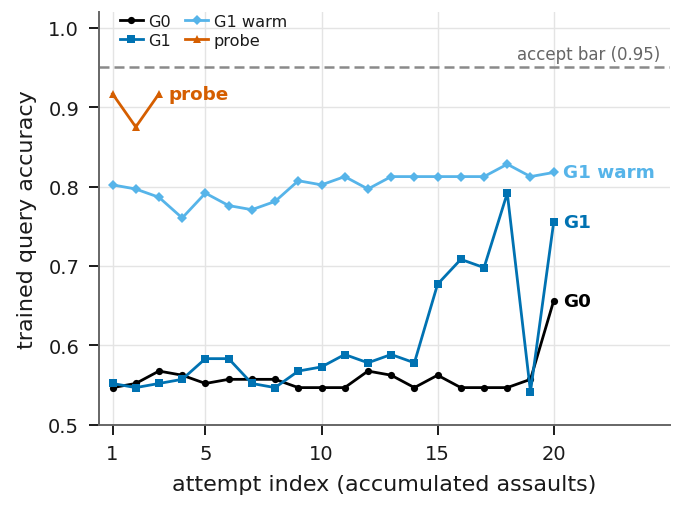
\includegraphics[keepaspectratio]{../../figures/fig3_spirals.png}}

\emph{Figure S1: Historical two-spirals query trajectories for G0, G1, the warm G1 continuation, and the interrupted probe. No arm crosses 0.95.}

\pandocbounded{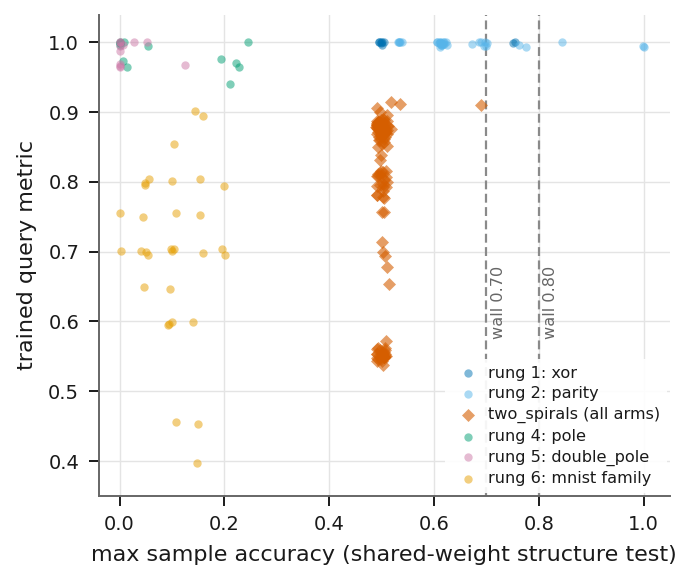
\includegraphics[keepaspectratio]{../../figures/fig4_wall.png}}

\emph{Figure S2: Trained performance versus shared-weight topology performance for historical champions. The two-spirals rows cluster near chance on the structural axis even when fitted performance rises.}

\section{Appendix F: July 12 Pre-Change Full-Ladder Run}\label{appendix-f-july-12-pre-change-full-ladder-run}

The July 12 preflight completed 180 of 180 tasks in 49,311.5 task-seconds and 3,987 generations. Outcomes were 74 evolved, 64 failed, 36 library hits, 4 refinements, and 2 decompositions. Held-out values were recorded for 137 tasks. Eighty-four entries were created; 69 remained after garbage collection. Held-out query accuracy is primary in the table below. \texttt{N/A} means no value was recorded.

\begin{longtable}[]{@{}
  >{\raggedleft\arraybackslash}p{(\linewidth - 18\tabcolsep) * \real{0.1000}}
  >{\raggedleft\arraybackslash}p{(\linewidth - 18\tabcolsep) * \real{0.1000}}
  >{\raggedleft\arraybackslash}p{(\linewidth - 18\tabcolsep) * \real{0.1000}}
  >{\raggedleft\arraybackslash}p{(\linewidth - 18\tabcolsep) * \real{0.1000}}
  >{\raggedleft\arraybackslash}p{(\linewidth - 18\tabcolsep) * \real{0.1000}}
  >{\raggedleft\arraybackslash}p{(\linewidth - 18\tabcolsep) * \real{0.1000}}
  >{\raggedleft\arraybackslash}p{(\linewidth - 18\tabcolsep) * \real{0.1000}}
  >{\raggedleft\arraybackslash}p{(\linewidth - 18\tabcolsep) * \real{0.1000}}
  >{\raggedleft\arraybackslash}p{(\linewidth - 18\tabcolsep) * \real{0.1000}}
  >{\raggedleft\arraybackslash}p{(\linewidth - 18\tabcolsep) * \real{0.1000}}@{}}
\toprule\noalign{}
\begin{minipage}[b]{\linewidth}\raggedleft
Rung
\end{minipage} & \begin{minipage}[b]{\linewidth}\raggedleft
Tasks
\end{minipage} & \begin{minipage}[b]{\linewidth}\raggedleft
Q cov.
\end{minipage} & \begin{minipage}[b]{\linewidth}\raggedleft
Q max
\end{minipage} & \begin{minipage}[b]{\linewidth}\raggedleft
Q mean
\end{minipage} & \begin{minipage}[b]{\linewidth}\raggedleft
S max
\end{minipage} & \begin{minipage}[b]{\linewidth}\raggedleft
S mean
\end{minipage} & \begin{minipage}[b]{\linewidth}\raggedleft
OK
\end{minipage} & \begin{minipage}[b]{\linewidth}\raggedleft
Fail
\end{minipage} & \begin{minipage}[b]{\linewidth}\raggedleft
s
\end{minipage} \\
\midrule\noalign{}
\endhead
\bottomrule\noalign{}
\endlastfoot
1 & 10 & 10/10 & 1.0000 & 1.0000 & 1.0000 & 1.0000 & 10 & 0 & 10.7 \\
2 & 10 & 10/10 & 1.0000 & 0.9846 & 1.0000 & 1.0000 & 10 & 0 & 412.9 \\
3 & 10 & 0/10 & N/A & N/A & 0.5670 & 0.5567 & 0 & 10 & 2133.9 \\
4 & 10 & 10/10 & 1.0000 & 0.9525 & 1.0000 & 0.9797 & 10 & 0 & 251.4 \\
5 & 10 & 10/10 & 0.9833 & 0.9600 & 0.9917 & 0.9700 & 10 & 0 & 111.2 \\
6 & 10 & 10/10 & 0.7500 & 0.5100 & 1.0000 & 0.9838 & 10 & 0 & 551.6 \\
7 & 10 & 8/10 & 0.3000 & 0.1531 & 1.0000 & 0.7350 & 6 & 4 & 3618.0 \\
8 & 10 & 10/10 & 0.7692 & 0.3769 & 1.0000 & 0.9392 & 7 & 3 & 2156.6 \\
9 & 10 & 7/10 & 0.6923 & 0.4945 & 1.0000 & 0.7725 & 3 & 7 & 5816.1 \\
10 & 10 & 10/10 & 0.8462 & 0.6538 & 1.0000 & 0.9510 & 9 & 1 & 2218.3 \\
11 & 10 & 5/10 & 0.0000 & 0.0000 & 0.9020 & 0.4490 & 0 & 10 & 6096.6 \\
12 & 10 & 10/10 & 0.9993 & 0.9840 & 0.9993 & 0.9847 & 10 & 0 & 1336.1 \\
13 & 10 & 1/10 & 0.1790 & 0.1790 & 0.7194 & 0.5996 & 0 & 10 & 6151.2 \\
14 & 10 & 0/10 & N/A & N/A & 0.9344 & 0.7453 & 0 & 10 & 3871.7 \\
15 & 10 & 10/10 & 0.9877 & 0.9846 & 0.9891 & 0.9846 & 10 & 0 & 735.3 \\
16 & 10 & 6/10 & 0.9231 & 0.8921 & 0.9597 & 0.9150 & 1 & 9 & 6326.0 \\
17 & 10 & 10/10 & 0.2308 & 0.1077 & 1.0000 & 1.0000 & 10 & 0 & 6211.6 \\
18 & 10 & 10/10 & 0.8438 & 0.5128 & 1.0000 & 0.9994 & 10 & 0 & 1302.2 \\
\end{longtable}

The table shows strong historical query results on rungs 1, 2, 4, 12, and 15, alongside severe gaps on images, PGM, and ARC. The ARC numbers are held-out cell-level accuracy. No exact-grid result was recorded. Deadline counters concentrated in upper rungs and were sampled only at cooperative boundaries. The persisted v1 router reached 5.3 GiB, dominated by wide adapters and heads.

The routed transcript often reached high adapter-space scores but lost accuracy during distillation. That is evidence of correct escalation plus insufficient executable parent wiring in that code era, not an ARC-specific router failure. Compact port maps, executable handoff, sharded routing, lifecycle decay, content-addressed archives, and counterfactual motif labels were implemented afterward. A matched rerun is required to evaluate their effect.

\section{Appendix G: July 15 Current-Method Canary}\label{appendix-g-july-15-current-method-canary}

\subsection{G.1 Complete root-task table}\label{g1-complete-root-task-table}

The canary completed all 18 scheduled roots in 720 generations and 6,925.5 recorded task-seconds. Query coverage was 16/18. Mean query accuracy over available rows was 0.6626; mean support accuracy over available rows was 0.8312; the paired mean support-minus-query gap was 0.1686. Outcome labels were 9 evolved, 2 decomposed, and 7 failed.

\begin{longtable}[]{@{}
  >{\raggedleft\arraybackslash}p{(\linewidth - 12\tabcolsep) * \real{0.1429}}
  >{\raggedright\arraybackslash}p{(\linewidth - 12\tabcolsep) * \real{0.1429}}
  >{\raggedright\arraybackslash}p{(\linewidth - 12\tabcolsep) * \real{0.1429}}
  >{\raggedleft\arraybackslash}p{(\linewidth - 12\tabcolsep) * \real{0.1429}}
  >{\raggedleft\arraybackslash}p{(\linewidth - 12\tabcolsep) * \real{0.1429}}
  >{\raggedleft\arraybackslash}p{(\linewidth - 12\tabcolsep) * \real{0.1429}}
  >{\raggedleft\arraybackslash}p{(\linewidth - 12\tabcolsep) * \real{0.1429}}@{}}
\toprule\noalign{}
\begin{minipage}[b]{\linewidth}\raggedleft
Rung
\end{minipage} & \begin{minipage}[b]{\linewidth}\raggedright
Task family
\end{minipage} & \begin{minipage}[b]{\linewidth}\raggedright
Outcome
\end{minipage} & \begin{minipage}[b]{\linewidth}\raggedleft
Support
\end{minipage} & \begin{minipage}[b]{\linewidth}\raggedleft
Query
\end{minipage} & \begin{minipage}[b]{\linewidth}\raggedleft
Gens
\end{minipage} & \begin{minipage}[b]{\linewidth}\raggedleft
s
\end{minipage} \\
\midrule\noalign{}
\endhead
\bottomrule\noalign{}
\endlastfoot
1 & XOR & evolved & 1.0000 & 1.0000 & 2 & 2.0 \\
2 & Parity & evolved & 0.9804 & 0.9231 & 15 & 3.8 \\
3 & Two spirals & failed & 0.5515 & 0.5000 & 33 & 19.5 \\
4 & Pole & evolved & 0.9875 & 0.9750 & 2 & 2.6 \\
5 & Double pole & evolved & 0.9958 & 0.9833 & 3 & 3.0 \\
6 & MNIST & evolved & 1.0000 & 0.6500 & 10 & 1.2 \\
7 & CIFAR-10 & evolved & 1.0000 & 0.1500 & 39 & 170.5 \\
8 & ECG & failed & 0.5882 & 0.7692 & 8 & 1000.1 \\
9 & Satellite & evolved & 1.0000 & 0.6923 & 133 & 530.4 \\
10 & NinaPro & evolved & 0.9608 & 0.8462 & 15 & 122.9 \\
11 & Spherical & failed & 0.2157 & 0.0000 & 10 & 907.9 \\
12 & Cosmic & decomp. & 0.9848 & 0.9837 & 45 & 427.6 \\
13 & Darcy Flow & failed & 0.1735 & 0.1781 & 34 & 301.6 \\
14 & Psicov & failed & N/A & N/A & 0 & 1232.8 \\
15 & FSD50K & evolved & 0.9615 & 0.8742 & 10 & 24.1 \\
16 & DeepSEA & failed & 0.8998 & 0.8761 & 6 & 925.0 \\
17 & PGM & failed & N/A & N/A & 0 & 1046.4 \\
18 & ARC & decomp. & 1.0000 & 0.2000 & 31 & 204.0 \\
\end{longtable}

Runtime success is support-side. MNIST, CIFAR, and ARC illustrate why outcome counts cannot replace held-out results. ECG has a higher query than support score because they are finite, separate samples and the support optimizer did not clear its bar. Psicov and PGM both record \path{time_limit_before_evaluation}; their missing values are not failures scored as zero.

\subsection{G.2 Strategy and persistence traces}\label{g2-strategy-and-persistence-traces}

The root selected paths were six composition, seven direct, three routed, and two deadline outcomes. Five deadline markers were recorded. Stage totals overlap because nested recursion contributes to more than one conceptual bucket; they should not be summed as disjoint wall time.

The cold library admitted 23 entries and removed none. It contains 7 modules and 16 compositions: 7 level-1, 5 level-2, 5 level-3, 4 level-4, 1 level-5, and 1 level-6 entry. All were live at the freeze. The router knew 17 active vertex keys at the end. Three router edges expired, while no vertex expired or revived and no library entry retired for inactivity.

At root level, routed handoff counts appeared on ECG, NinaPro, Spherical, Cosmic, and ARC. Cosmic recovered from a router score of 0.9848 and distilled score 0.9183 to an executable parent support score of 0.9848 after composition/decomposition. ARC recovered from router score 1.0 and distilled score 0.8294 to support score 1.0. These recovery fields show that below-bar distilled artifacts were carried forward. They do not show that handoff caused the final score, and ARC\textquotesingle s query remained 0.20.

The run had no root refinement or library-hit outcome because each rung contributed one cold task. The summary\textquotesingle s nested counters include subtask hits and admissions; they should not be mistaken for repeated root-family evidence. No topology duplicate counter fired, no entry was garbage-collected, and no motif discovery run was attached.

\pandocbounded{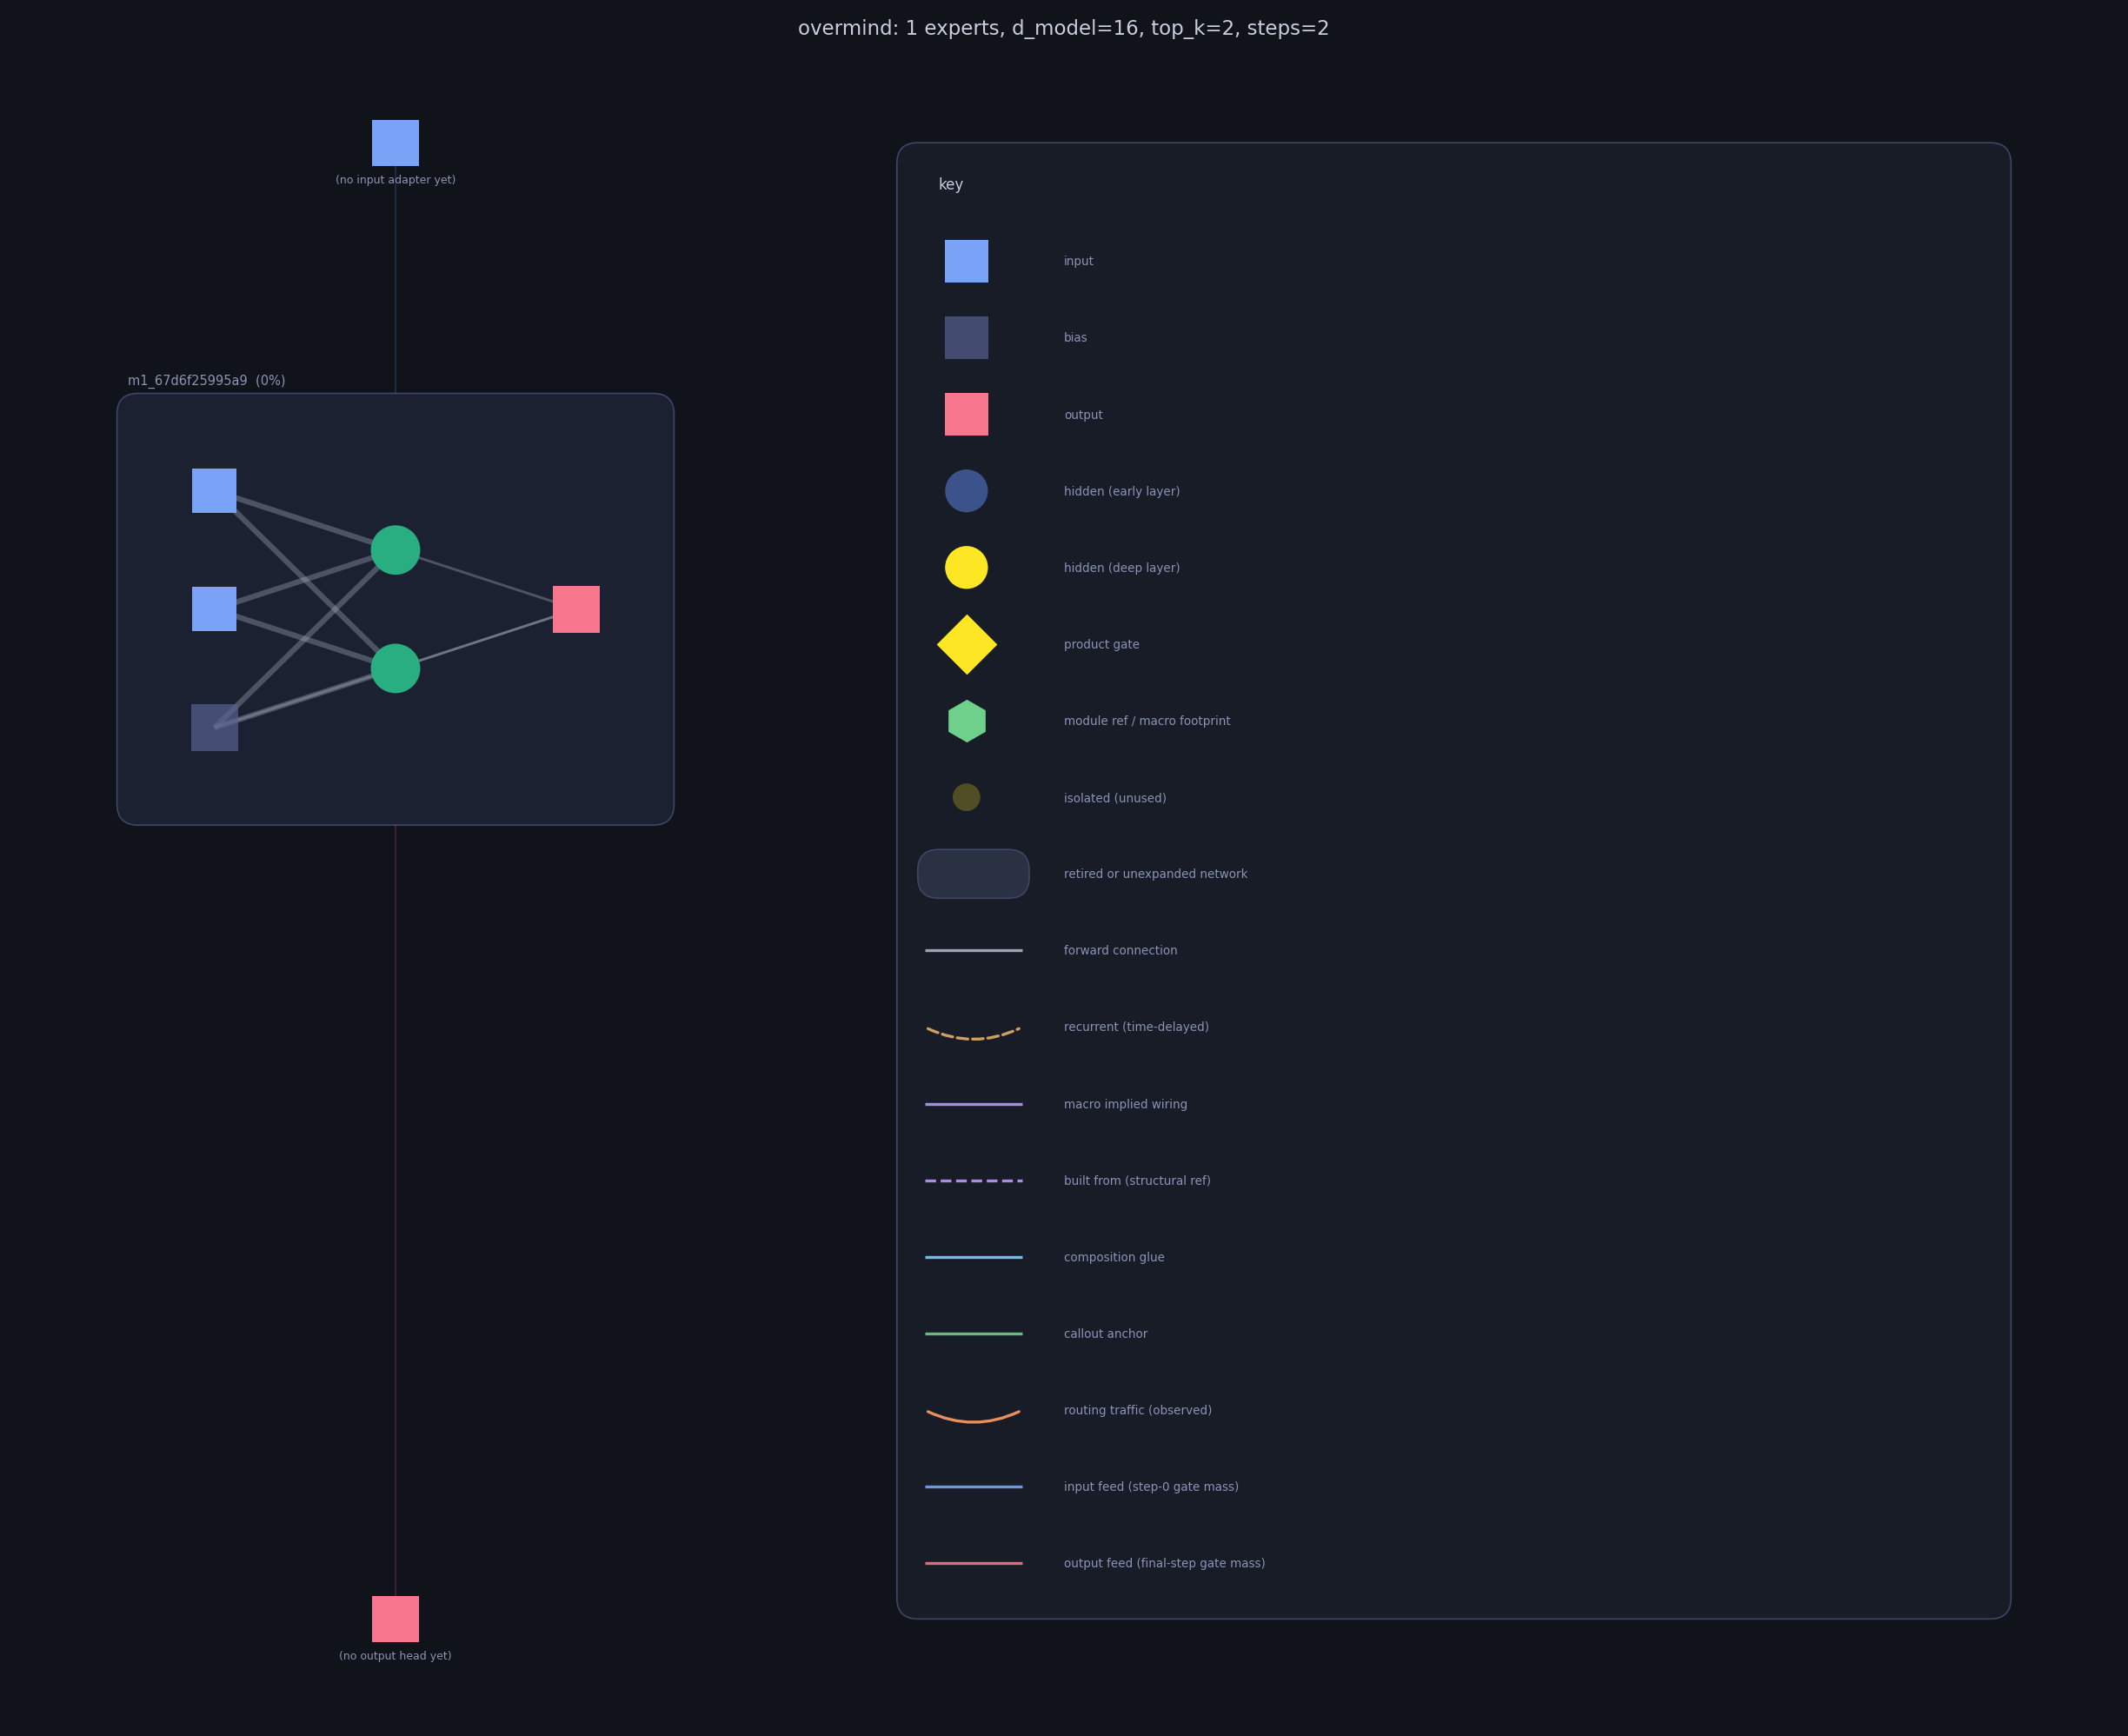
\includegraphics[keepaspectratio]{../../figures/fig5a_overmind.png}}

\emph{Figure S3: Historical overmind portrait retained as a library visualization example. It is not the July 15 library and is not used as evidence for July 15 route traffic.}

\section{Appendix H: Descriptive Library Structure}\label{appendix-h-descriptive-library-structure}

The historical frozen flagship library contained 24 live mineable entries among 35 retained index entries after garbage collection. Its raw census found 358 distinct size-3/4 module motifs: 135 mixed, 121 macro-bearing, 61 gated, 32 gated-plus-macro, and 9 uniform-tanh, plus one composition motif. The most frequent appeared in 19 of 22 scanned modules. A smaller warm snapshot contained 138 distinct motifs across nine live modules.

These are canonical frequency counts. They show repeated graph fragments and provide grammar candidates. They do not establish independent origin, performance association, or function. In particular, macro-bearing frequency is expected in a library already selected for hierarchical reuse. The old atlas is therefore relabeled descriptive.

\pandocbounded{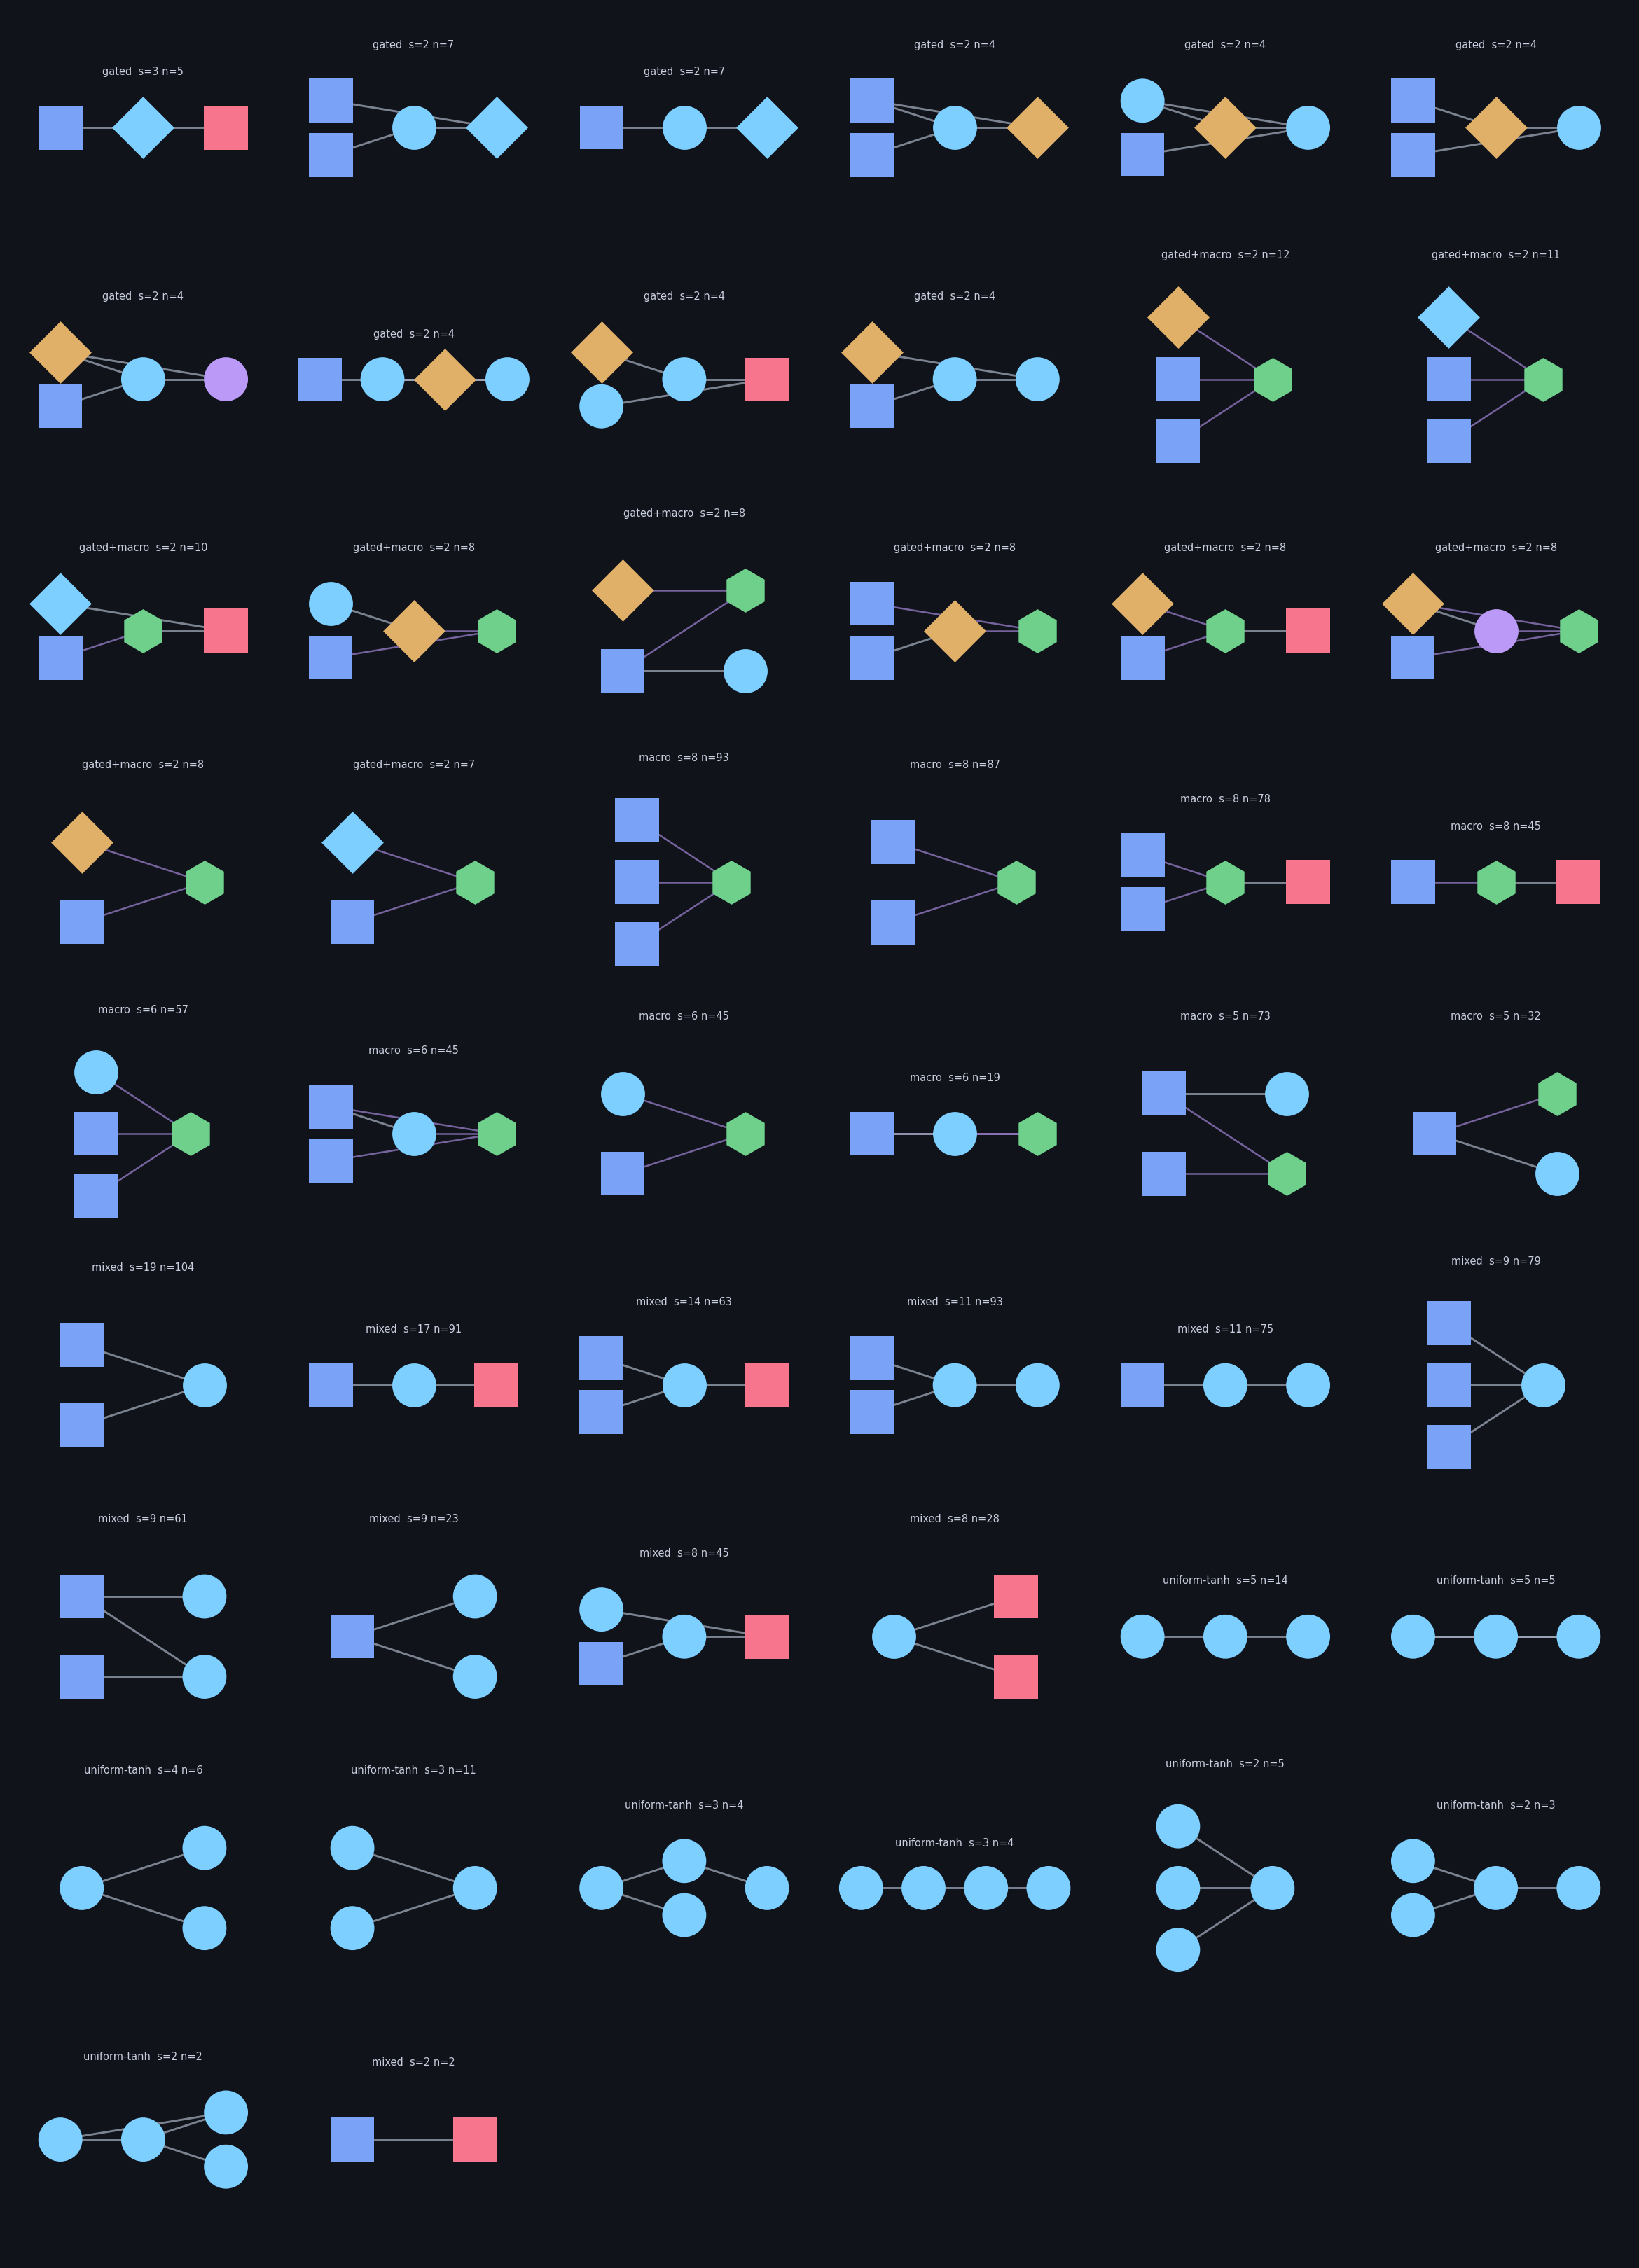
\includegraphics[keepaspectratio]{../../figures/fig6_motifs.png}}

\emph{Figure S4: Historical descriptive motif atlas. Color and count summarize canonical recurrence only; no panel is claimed as a discovered architectural primitive.}

Two historical artifacts illustrate why causal tests matter. A warm two-spirals network explicitly repeated a sin/product macro six times, which looks visually modular but could be redundant. A level-3 parity chain reused lower-level modules, which proves reference nesting but not that every referenced edge is necessary. The counterfactual protocol now asks whether frozen removal harms accuracy more than matched controls and whether the effect replicates across independent roots.

\pandocbounded{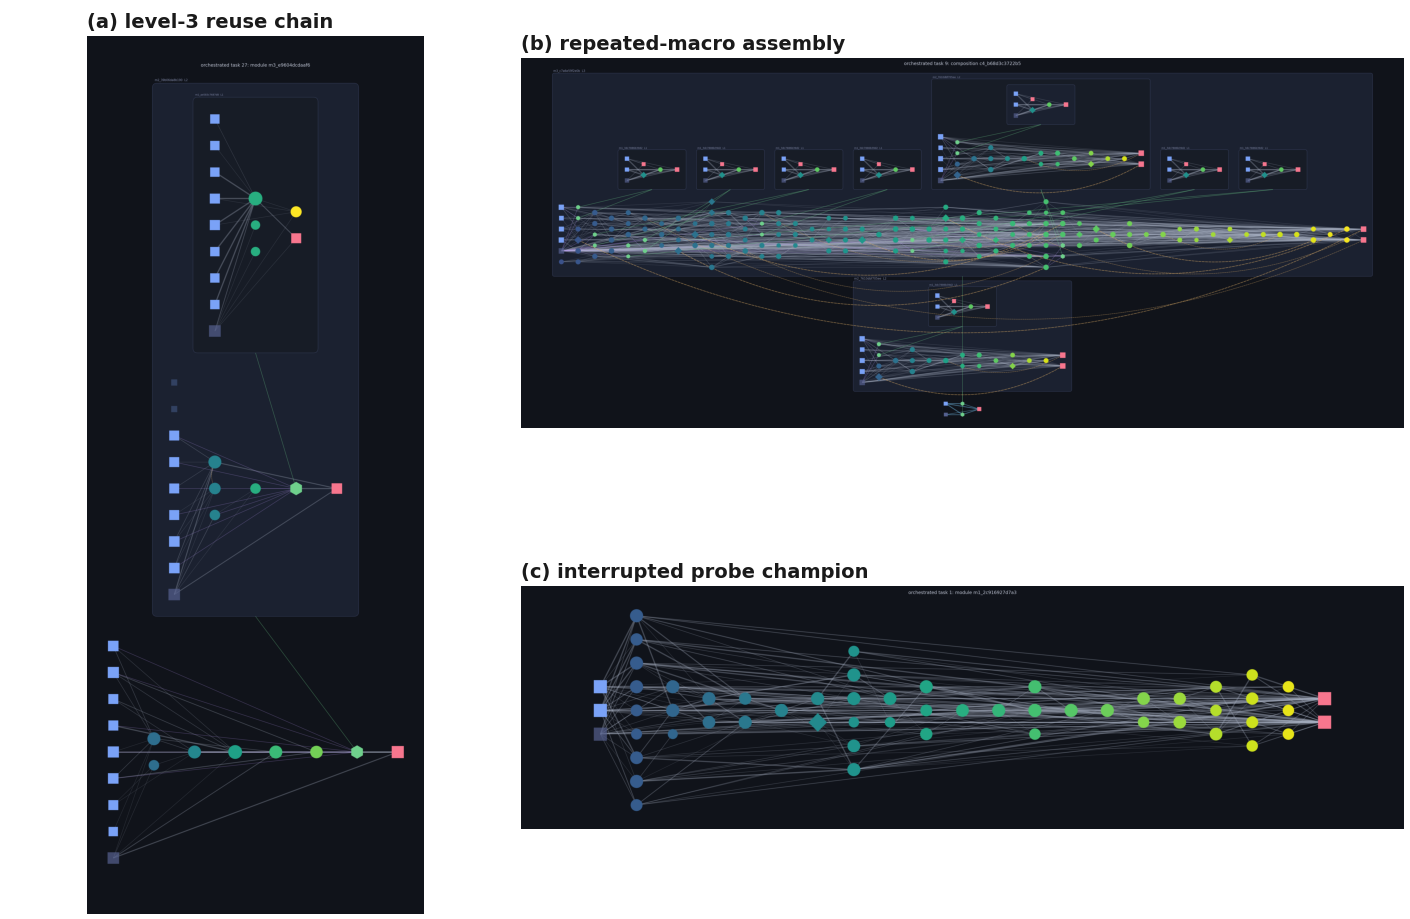
\includegraphics[keepaspectratio]{../../figures/fig5e_artifact_triptych.png}}

\emph{Figure S5: Historical library artifacts: repeated macro assembly, a three-level reference chain, and the best interrupted two-spirals probe champion. They are mechanistic illustrations, not architectural-discovery evidence.}

\section{Appendix I: Engineering and Resource Postmortems}\label{appendix-i-engineering-and-resource-postmortems}

\subsection{I.1 Resource estimation}\label{i1-resource-estimation}

The allocator estimates host and device residency before each stage. Host limits account for process/cgroup memory and a configured reserve. Device limits account for free CUDA memory and reserve. Direct populations charge their actual population and concurrency mode. Composition populations charge compact glue and resident modules. Routed distillation charges one selected pathway rather than multiplying it by a composition population. Fixed caps, where positive, retain precedence over adaptive fractions.

These are deterministic estimates, not reservations. They cannot prevent allocator fragmentation or an unexpectedly expensive inner operation. Their purpose is to decline obviously impossible work before constructing it and to record the arithmetic behind that decision.

\subsection{I.2 Historical incidents}\label{i2-historical-incidents}

Four incidents shaped the present instrumentation.

\begin{enumerate}
\def\labelenumi{\arabic{enumi}.}
\tightlist
\item
  A CIFAR run spent approximately eight hours at low CPU because geometry mutation performed a main-thread pair sweep. Per-stage timing identified mutation rather than device training; the replacement was pinned against a reference implementation.
\item
  Composition consumed 849 of 860 seconds per task after a cycle-repair helper regressed into repeated constructors. The repaired helper measured approximately 0.06 ms per call.
\item
  A 409,600-input task entered an expensive first generation before any deadline seam existed. One genome required approximately 2.6 seconds and 0.79 GB; the population implied minutes and tens of gigabytes before the loop could check time. Preflight resource guards were added.
\item
  A July 12 Psicov task with 13,966,425 inputs and 245,025 outputs required an estimated 113,936,625 rank-8 glue values per minimal candidate in the historical representation, approximately 3.40 GiB per candidate and 163 GiB for a population of 48. The parent was killed; worker broken pipes were secondary. Compact port maps and stage-aware resource accounting address the representation failure, but a wide task remains intrinsically expensive.
\end{enumerate}

The July 12 v1 router\textquotesingle s 5.3 GiB state was another representation cost. The July 15 v2 archive separates its 105,020-byte resident core from approximately 287 MiB of on-demand shards. This is a substantial storage-layout difference, but the campaigns are not a controlled memory benchmark.

\subsection{I.3 Deadlines and shutdown}\label{i3-deadlines-and-shutdown}

Task and recursive deadlines are cooperative. The orchestrator checks them between strategies, generations, and other safe seams. It cannot safely interrupt an arbitrary tensor operation or optimizer update without risking corrupted state. Five July 15 roots reached deadline markers, and some elapsed times overshot nominal limits before the active unit returned.

Escape requests set the same cooperative stop signal but differ from time-budget failure: no artificial deadline failure is recorded, no blind query evaluation begins after the request, and the normal finalization writes reports, checkpoints, library renders, and archive status \texttt{stopped}. Terminal state is restored even when the run exits through an error path. Ctrl-C remains available for immediate interruption and is recorded as a crash.

\subsection{I.4 External archives}\label{i4-external-archives}

Archive format v2 stores a manifest whose file records point to content-addressed objects. A run snapshot that shares unchanged library or router files with an earlier snapshot uploads only new objects. List, verify, and restore remain compatible with v1 archives. Restore verifies every object hash, assembles a temporary tree, and atomically installs the destination only after the complete tree passes verification.

\section{Appendix J: Broader Impact and Claim Discipline}\label{appendix-j-broader-impact-and-claim-discipline}

ArdEVO searches small supervised neural systems under fixed tasks, verifiers, and budgets. Its durable artifacts are inert serialized networks and compositions. They do not write code or act outside the runtime. The nearest-term risks are scientific and operational: warm-library provenance can inflate results; broad support fitting can be mistaken for held-out capability; and structured cell accuracy can be mistaken for task-exact reasoning. The evidence and report pipeline is designed to make those errors visible.

Longer-term systems that select their own objectives, modify their implementation, or operate persistently in open environments would present a different risk profile. The current architecture could be one component of such a system because it accumulates reusable structure, but it does not implement those capabilities. Likewise, neither evolved structure nor benchmark performance is evidence of consciousness. Any future claim about objectness, selfhood, qualia, or sentience would require operational definitions and experiments absent here.

The release remains a research artifact. Submission-quality claims require the pending multi-seed campaign, matched external baselines, exact structured metrics, a pinned executable revision, and a durable public evidence deposit. Until those conditions are met, the canaries should be read as transparent capability probes and engineering evidence, not as a leaderboard result.

\begin{center}\rule{0.5\linewidth}{0.5pt}\end{center}

\section{References}\label{references}

Alet, F., Lozano-Perez, T., and Kaelbling, L. P. (2018). Modular meta-learning. \emph{Conference on Robot Learning (CoRL)}. arXiv:1806.10166.

Andreas, J., Rohrbach, M., Darrell, T., and Klein, D. (2016). Neural module networks. \emph{CVPR 2016}. arXiv:1511.02799.

ARC Prize Foundation (2026). ARC-AGI-3: A new challenge for frontier agentic intelligence. arXiv:2603.24621.

Barrett, D. G. T., Hill, F., Santoro, A. S., Morcos, A. S., and Lillicrap, T. (2018). Measuring abstract reasoning in neural networks. \emph{ICML 2018}. arXiv:1807.04225.

Bowers, M., Olausson, T. X., Wong, L., Grand, G., Tenenbaum, J. B., Ellis, K., and Solar-Lezama, A. (2023). Top-down synthesis for library learning. \emph{POPL 2023}. arXiv:2211.16605.

Chollet, F. (2019). On the measure of intelligence. arXiv:1911.01547.

Clune, J. (2019). AI-GAs: AI-generating algorithms, an alternate paradigm for producing general artificial intelligence. arXiv:1905.10985.

Ecoffet, A., Huizinga, J., Lehman, J., Stanley, K. O., and Clune, J. (2021). First return, then explore. \emph{Nature}, 590:580-586.

Ellis, K., Wong, C., Nye, M., Sable-Meyer, M., Cary, L., Morales, L., Hewitt, L., Solar-Lezama, A., and Tenenbaum, J. B. (2021). DreamCoder: Bootstrapping inductive program synthesis with wake-sleep library learning. \emph{PLDI 2021}. arXiv:2006.08381.

Elsken, T., Metzen, J. H., and Hutter, F. (2019). Neural architecture search: A survey. \emph{JMLR}, 20(55):1-21. arXiv:1808.05377.

Gaier, A., and Ha, D. (2019). Weight agnostic neural networks. \emph{NeurIPS 2019}. arXiv:1906.04358.

Hinton, G. E., and Nowlan, S. J. (1987). How learning can guide evolution. \emph{Complex Systems}, 1(3):495-502.

Jacobs, R. A., Jordan, M. I., Nowlan, S. J., and Hinton, G. E. (1991). Adaptive mixtures of local experts. \emph{Neural Computation}, 3(1):79-87.

Lehman, J., and Stanley, K. O. (2011). Abandoning objectives: Evolution through the search for novelty alone. \emph{Evolutionary Computation}, 19(2):189-223.

Liu, H., Simonyan, K., and Yang, Y. (2019). DARTS: Differentiable architecture search. \emph{ICLR 2019}. arXiv:1806.09055.

McCloskey, M., and Cohen, N. J. (1989). Catastrophic interference in connectionist networks: The sequential learning problem. \emph{Psychology of Learning and Motivation}, 24:109-165.

Mendez, J. A., and Eaton, E. (2021). Lifelong learning of compositional structures. \emph{ICLR 2021}. arXiv:2007.07732.

Meyerson, E., and Miikkulainen, R. (2018). Beyond shared hierarchies: Deep multitask learning through soft layer ordering. \emph{ICLR 2018}. arXiv:1711.00108.

Miikkulainen, R., Liang, J., Meyerson, E., Rawal, A., Fink, D., Francon, O., Raju, B., Shahrzad, H., Navruzyan, A., Duffy, N., and Hodjat, B. (2017). Evolving deep neural networks. arXiv:1703.00548.

Mouret, J.-B., and Clune, J. (2015). Illuminating search spaces by mapping elites. arXiv:1504.04909.

Pugh, J. K., Soros, L. B., and Stanley, K. O. (2016). Quality diversity: A new frontier for evolutionary computation. \emph{Frontiers in Robotics and AI}, 3:40.

Real, E., Aggarwal, A., Huang, Y., and Le, Q. V. (2019). Regularized evolution for image classifier architecture search. \emph{AAAI 2019}. arXiv:1802.01548.

Real, E., Moore, S., Selle, A., Saxena, S., Suematsu, Y. L., Tan, J., Le, Q., and Kurakin, A. (2017). Large-scale evolution of image classifiers. \emph{ICML 2017}. arXiv:1703.01041.

Rusu, A. A., Rabinowitz, N. C., Desjardins, G., Soyer, H., Kirkpatrick, J., Kavukcuoglu, K., Pascanu, R., and Hadsell, R. (2016). Progressive neural networks. arXiv:1606.04671.

Shazeer, N., Mirhoseini, A., Maziarz, K., Davis, A., Le, Q., Hinton, G., and Dean, J. (2017). Outrageously large neural networks: The sparsely-gated mixture-of-experts layer. \emph{ICLR 2017}. arXiv:1701.06538.

Stanley, K. O. (2007). Compositional pattern producing networks: A novel abstraction of development. \emph{Genetic Programming and Evolvable Machines}, 8(2):131-162.

Stanley, K. O., Clune, J., Lehman, J., and Miikkulainen, R. (2019). Designing neural networks through neuroevolution. \emph{Nature Machine Intelligence}, 1:24-35.

Stanley, K. O., D\textquotesingle Ambrosio, D. B., and Gauci, J. (2009). A hypercube-based encoding for evolving large-scale neural networks. \emph{Artificial Life}, 15(2):185-212.

Stanley, K. O., Lehman, J., and Soros, L. (2017). Open-endedness: The last grand challenge you\textquotesingle ve never heard of. \emph{O\textquotesingle Reilly Radar}.

Stanley, K. O., and Miikkulainen, R. (2002). Evolving neural networks through augmenting topologies. \emph{Evolutionary Computation}, 10(2):99-127.

Tu, R., Roberts, N., Khodak, M., Shen, J., Sala, F., and Talwalkar, A. (2022). NAS-Bench-360: Benchmarking neural architecture search on diverse tasks. \emph{NeurIPS 2022 Datasets and Benchmarks}. arXiv:2110.05668.

Veniat, T., Denoyer, L., and Ranzato, M. (2021). Efficient continual learning with modular networks and task-driven priors. \emph{ICLR 2021}. arXiv:2012.12631.

Wang, G., Xie, Y., Jiang, Y., Mandlekar, A., Xiao, C., Zhu, Y., Fan, L., and Anandkumar, A. (2023). Voyager: An open-ended embodied agent with large language models. arXiv:2305.16291.

Wang, R., Lehman, J., Clune, J., and Stanley, K. O. (2019). Paired open-ended trailblazer (POET): Endlessly generating increasingly complex and diverse learning environments and their solutions. arXiv:1901.01753.

Wang, R., Lehman, J., Rawal, A., Zhi, J., Li, Y., Clune, J., and Stanley, K. O. (2020). Enhanced POET: Open-ended reinforcement learning through unbounded invention of learning challenges and their solutions. \emph{ICML 2020}. arXiv:2003.08536.

Whitley, D., Gordon, V. S., and Mathias, K. (1994). Lamarckian evolution, the Baldwin effect and function optimization. \emph{PPSN III}, LNCS 866, 6-15.

\end{document}
